\documentclass[12pt,titlepage]{report}
\usepackage[italian]{babel}
\usepackage{url,amsfonts,epsfig}
\usepackage[utf8]{inputenc}
\usepackage{amsmath}
\usepackage{float}
\usepackage{pgfplots}
\usepackage{caption}
\usepackage{algorithm2e}
\usepackage{listings}
\usepackage{color}
\usepackage{array}
\usepackage{geometry}
\usepackage[normalem]{ulem}
\usepackage{graphicx}
\usepackage{gensymb}
\usepackage{enumitem}
\usepackage{verbatim}
\usepackage{siunitx}



\lstset
{ %Formatting for code in appendix
    language=Python,
    basicstyle=\footnotesize,
    numbers=left,
    stepnumber=1,
    showstringspaces=false,
    tabsize=1,
    breaklines=true,
    breakatwhitespace=false,
}

\renewcommand*{\lstlistingname}{Listato}
\input{custom_commands.tex}

\title{Esplorazione adattiva di uno sciame di droni per il rilevamento di target distribuiti}
\author{Domenico Minici}
\date{19 luglio 2019}

\setcounter{secnumdepth}{3}
\setcounter{tocdepth}{3}
\begin{document}



\makeatletter
\newgeometry{left=3.5cm,bottom=2.5cm}

\begin{titlepage}
    \newcommand{\HRule}{\rule{\linewidth}{0.5mm}}
    
    \center 
    \textsc{\LARGE Università Di Pisa }\\[0.3cm]

    \vspace{1cm}
    
\includegraphics[scale=0.5]{img/logo.png}
    \vspace{1cm}
  
    \textsc{\Large Tesi Magistrale in }\\[0.5cm]
    \textsc{\Large Computer Engineering }\\[1.5cm]
  
    \HRule \\[0.4cm]
    { \huge \bfseries \@title }\\[0.03cm] 
    \HRule \\[1.5cm]
    
    \begin{minipage}{0.4\textwidth}
    \begin{flushleft} \large
    \emph{Relatori:}\\
    Mario G.C.A. Cimino\\
    Gigliola Vaglini
    \end{flushleft}
    \end{minipage}
    ~
    \begin{minipage}{0.4\textwidth}
    \begin{flushright} \large
    \emph{Candidato:} \\
    \@author \\ 
    \vspace{1.2\baselineskip}
    \end{flushright}
    \end{minipage}\\[1cm]
    
    \vfill

    {\large \@date }\\[1cm]

   
\end{titlepage}

\restoregeometry

\newgeometry{left=3.5cm}

\cleardoublepage
\thispagestyle{empty}
\vspace*{\stretch{1}}
\begin{flushleft}
\itshape A zio Saverio,\\
un grande Uomo ed esempio da seguire,\\
un secondo padre.
\end{flushleft}
\vspace{\stretch{2}}
\cleardoublepage

\restoregeometry


\newgeometry{left=3.5cm}
\pagenumbering{Roman}
\newgeometry{left=3.5cm,top=2cm}
\chapter*{Abstract}

Questa tesi si concentra sul problema del coordinamento di più UAV per il rilevamento e il tracking di target distribuiti, in diversi contesti tecnologici e ambientali. 
\`E stato implementato un ambiente di simulazione, basato sulla tecnologia UAV disponibile in commercio e su scenari reali. 
L'approccio analizzato si basa sul concetto di comportamento dello sciame in sistemi multi-agente, cioè un team di UAV autoformato e auto-coordinato che si adatta a layout ambientali specifici della missione. 
La formazione e la coordinazione degli sciami sono ispirati da meccanismi biologici.
Questi meccanismi, opportunamente combinati, permettono di trovare il giusto equilibrio tra ricerca globale (\textit{exploration}) e ricerca locale (\textit{exploitation}) nell'ambiente. 
Il simulatore è provvisto di un modulo software per l'integrazione di algoritmi basati sulle strategie presenti in letteratura.
L'obiettivo del simulation tested proposto è quello di adattare le strategie integrate attraverso un meccanismo di ottimizzazione parametrica, eseguito su architetture parallele, al fine di condurre una valutazione delle performance di tali strategie e di effettuare un'analisi comparativa, basata su diversi test di simulazione, per identificare i punti chiave da sfruttare e migliorare nei lavori futuri. 
Le strategie analizzate in questa tesi sono: (i) Algoritmo Stigmergy-Flocking-Evolution (SFE), basato su meccanismi biologici come il flocking e la stigmergia; (ii) Firefly-based team strategy for robot recruitment, basato sul comportamento delle lucciole; (iii) Particle swarm optimization for robot recruitment, basato sul comportamento di agenti in stormo; (iv) Artificial bee colony algorithm for robot recruitment, basato invece sul comportamento delle api nella ricerca di fonti di cibo.
L'adattamento dello sciame è sostenuto da algoritmi evolutivi con l'obiettivo di massimizzare il numero di bersagli tracciati durante una missione o di ridurre al minimo il tempo per la scoperta del bersaglio. 
I risultati sperimentali dimostrano che l'ambiente permette una valutazione qualitativa e quantitativa delle performance ed un'importante ottimizzazione parametrica, grazie ad un meccanismo evolutivo basato su architetture parallele, delle strategie bio-ispirate analizzate.

\restoregeometry 
\restoregeometry

\newgeometry{left=3.5cm,top=2cm,bottom=2cm}
\tableofcontents
\restoregeometry

\newgeometry{left=3.5cm}
\pagenumbering{arabic}
\setlength{\parskip}{0.3cm}
\chapter{Introduzione}

Negli ultimi anni, sono state effettuate diverse ricerche orientate allo sviluppo di strumenti e metodi per il monitoraggio e le operazioni all’interno di scenari complessi. 
Le missioni all’interno di questi contesti sono generalmente classificate come “noiose, sporche e pericolose” (categorizzazione delle “three Ds”, dall’inglese dull, dirty and dangerous), in quanto l’accesso a determinate zone risulta limitato, pericoloso o, in alcuni casi, impossibile, sia ad operatori umani che ai mezzi convenzionali.

Piattaforme aeree come gli UAV (Unmanned Aerial Vehicles), spesso chiamati droni, sono oggi la risposta più frequente alle esigenze di tali missioni, grazie ai recenti progressi tecnologici in materia di miniaturizzazione della batteria, di tecnologia di comunicazione, elaborazione e rilevamento \cite{whitehead2014remote}. 
In particolare, la categoria specifica per questa tipologia di operazioni è quella dei mini-UAV, droni di piccole dimensioni equipaggiati con strumenti di self-localization e sensing utilizzati per la raccolta dei dati necessari al completamento dei task prefissati.

L'individuazione e l'identificazione di un obiettivo sono elementi chiave in tutte le operazioni di cui sopra.
In alcune di esse, però, anche il tempo di completamento del task ricopre un ruolo fondamentale, basti pensare ad operazioni di ricerca e recupero di particolari target: in questa tipologia di task un’analisi dettagliata di tutto l’ambiente può rappresentare una strategia inefficiente. 
Un approccio sicuramente più appropriato potrebbe essere quello di effettuare una ricognizione veloce dell’area, con l’unico scopo di identificare i punti chiave da sottomettere, in un secondo momento, ad un'ispezione più accurata. 
In questo contesto, la qualità degli strumenti di sensing ha un impatto diretto sulle performance dell'intera missione \cite{bertuccelli2005robust}, così come il numero di attori utilizzati: completare tutte le operazioni con un singolo UAV può risultare rischioso (il drone è il nostro single point-of-failure) ed altamente costoso in termini di progettazione, costruzione e manutenzione del velivolo e dell'array di sensori su di esso presente.

L'utilizzo di uno sciame di mini-UAV, ed il conseguente approccio cooperativo che sfrutta gli strumenti di misurazione di tutti i velivoli, può minimizzare l'errore relativo all'identificazione dei target. 
I maggiori benefici che ne possono derivare sono robustezza, scalabilità e flessibilità e, per tale ragione, è necessario che ogni individuo dello sciame agisca ad un certo livello di autonomia ed esegua operazioni di sensing e comunicazione locali senza un controllo centralizzato o conoscenze globali della missione. 
L’elemento chiave del funzionamento di uno sciame di droni – in particolare, una delle principali ragioni per cui parliamo di sciame e non di gruppo – è la cooperazione tra gli individui, che permette di completare il task globale attraverso una serie di meccanismi di coordinazione ed esplorazione attuati dai singoli UAV. 
La principale ispirazione deriva proprio da osservazioni di animali sociali, quali formiche, api, pesci o uccelli, che riescono ad eseguire operazioni complesse di gruppo attraverso poche regole elementari, mostrando una sorta di conoscenza collettiva costituita con delle semplici interazioni locali \cite{brambilla2013swarm}.

Un meccanismo fondamentale di coordinamento dello sciame è la cosiddetta stigmergia \cite{sauter2005performance}. 
Attraverso questo processo, gli individui lasciano informazioni nell’ambiente in forma di feromoni, sostanze evaporabili diffuse localmente a cui altri individui reagiscono modificando il loro comportamento di conseguenza \cite{parunak2002digital}. 
Una strategia che permette l’organizzazione dei droni in sciami, invece, è il flocking, un comportamento emergente basato su semplici regole quali allineamento, separazione e coesione \cite{reynolds1987flocks}. 
Una forma simulata di feromone, la strategia di flocking ed una serie di meccanismi di evitamento di ostacoli, dunque, possono essere utilizzate per coordinare lo sciame e raggiungere l’obiettivo della missione.

Una volta introdotti gli attori principali del coordinamento di uno sciame di mini-UAV è necessario valutare tali meccanismi attraverso uno strumento di simulazione. 
Un simulatore di esplorazione dello sciame ha degli obiettivi diversi rispetto ad un simulatore di volo del drone: quest’ultimo si occupa di modellare aspetti di movimento o ambientali; quando trattiamo uno sciame, invece, la modellazione riguarda il sensing e le regole di comportamento che permettono ai singoli individui di collaborare ai fini del completamento di un particolare task. 
L’obiettivo di questo documento è quello di implementare un simulation testbed, all’interno del quale è possibile integrare diversi algoritmi al fine di valutarne le performance ed attuare un’analisi comparativa tra gli stessi.

Prima di passare ai dettagli implementativi dell’ambiente di simulazione verrà presentata, nel capitolo successivo, un’analisi sullo stato dell’arte relativo agli algoritmi bioispirati e sulle varie ricerche che hanno portato alle conoscenze odierne. 
Successivamente, verranno presentate in dettaglio le caratteristiche chiave degli algoritmi selezionati per la comparazione all’interno del testbed. 
Infine, verrà illustrata l’implementazione del simulatore, insieme all’algoritmo di Differential Evolution utilizzato per l’ottimizzazione parametrica ed ai risultati a contorno della nostra analisi.

\chapter{Stato dell'arte}

Molte ricerche sono state sviluppate nel campo della metaeuristica per la ricerca del target utilizzando uno sciame: queste ricerche sono caratterizzate per l'eterogeneità di obiettivi, metodologie e scenari. 
Alcune indagini recenti (ad esempio, \cite{senanayake2016search}) hanno tentato di creare una tassonomia per discutere le differenze qualitative tra gli approcci proposti. 
In questa sezione alcuni lavori rilevanti sono brevemente citati e riassunti per il lettore interessato.

Tra gli approcci di ispirazione biologica esistenti in letteratura, stigmergia e flocking sono ampiamente utilizzati per coordinare uno sciame di UAV in compiti di ricerca di target \cite{parunak2002digital}. 
Gli autori in \cite{sauter2005performance} hanno proposto uno schema di sciame basato sulla stigmergia, in cui feromoni virtuali sono depositati su una mappa feromonica e rilevati dagli agenti. 
In particolare, le decisioni relative ad azioni e movimenti sono prese dagli agenti camminatori, mentre gli agenti avatar si impegnano a fare stime in assenza di informazioni sul sensore. 
Lo schema è applicato a molti scenari, compresa l'acquisizione del target. 
In \cite{brust2017target} gli autori progettano una procedura di multi-hop clustering combinata con la stigmergia per fornire una soluzione ottimale ad un insieme di obiettivi, tra cui il rilevamento e il monitoraggio dei target. 
Inoltre, propongono un modello di feromoni che include feromoni attrattivi e repulsivi, per marcare rispettivamente i target rilevati e le aree visitate. 
Un'altra applicazione di questo tipo di modello di feromoni è proposta in \cite{atten2016uav}, per missioni simili.

Il flocking è stato proposto per la prima volta da Reynolds \cite{reynolds1987flocks}. 
Un esempio è proposto in \cite{vasarhelyi2014outdoor} dove gli autori presentano una strategia di coordinamento decentrato per gli UAV basata sul flocking. 
Questo meccanismo è utilizzato per mantenere gli UAV nel campo della comunicazione e per coordinarsi durante i loro task. 
In \cite{hauert2011reynolds} viene proposto un gruppo di UAV multipli ad ala fissa che volano ad una distanza relativamente grande l'uno dall'altro. 
Una strategia di flocking viene applicata anche in \cite{quintero2013flocking} dove gli UAV navigano autonomamente in un'area di ricerca.

Diversi lavori di ricerca hanno proposto miglioramenti per tali metaeuristiche biologiche \cite{bayindir2016review}. 
Queste, a differenza delle euristiche, non sono problem-dependent e possono essere utilizzate come strumenti generali per la risoluzione dei problemi. 
Ovviamente, una regolazione parametrica è necessaria per adattare una metaeuristica al task in questione ed una taratura di scarsa qualità può portare a risultati imprevedibili. 
Per esempio, la stigmergia con feromoni persistenti e con un ampio raggio di diffusione può attrarre troppi agenti e portare a ricerche inefficienti. 
Il flocking con un ampio raggio di visibilità può portare ad una formazione molto rigida. 
Poiché nei sistemi multi-agente l'interazione degli agenti non è semplicemente deducibile dalle proprietà dei componenti, un'importante tecnica per studiare le proprietà globali e il loro livello di prevedibilità è la simulazione che può essere utilizzata anche quando si propone una variante di una metaeuristica. 
I lavori che seguono riassumono alcune varianti di flocking e stigmergia utilizzate per i sistemi multi-UAVs.

In questo contesto, in \cite{paradzik2016multi} rispetto al modello a feromoni di ispirazione biologica, solitamente attrattivo/ripulsivo, gli autori codificano informazioni specifiche come sapori feromonici. 
In \cite{de2017fault} l'auto-organizzazione di uno sciame di UAV, impiegato in una missione di copertura territoriale, si ottiene consentendo la comunicazione a breve raggio tra UAV attraverso il gossiping. 
In \cite{qiu2017pigeon} gli autori propongono una strategia di coordinamento basata sul modello di flocking dei piccioni. 
Per evitare gli ostacoli, gli individui più alti nella gerarchia del flock sono informati sulla posizione degli ostacoli, fornendo una strategia di pianificazione del percorso basata su un campo di potenziale artificiale. 
In \cite{palmieri2017comparison} gli autori propongono diversi approcci basati su tre diversi algoritmi bio-ispirati per effettuare un confronto di metaeuristica applicata ad uno sciame di robot che deve completare una missione con l'obiettivo di minimizzare il consumo energetico.

La particolarità dell'approccio qui proposto è che le metaeuristiche del flocking e della stigmergia generano, insieme a rilevamento ed attuazione, una logica integrata che è parametrizzata nel suo insieme da un'ottimizzazione di Differential Evolution. 
Un processo di adattamento, infatti, può ricercare la migliore aggregazione delle metaeuristiche secondo la missione specifica e la misura delle prestazioni, che può essere testata nell'ambiente simulato, esplorando soluzioni normalmente impossibili da considerare in una progettazione convenzionale \cite{singh2017detection}, \cite{bloembergen2015evolutionary}.

Ciò è confermato da lavori di ricerca come \cite{cimino2015combining} in cui è necessario un meccanismo di adattamento che regola la coordinazione dello sciame per adattarsi al layout dello scenario attuale. 
Un altro esempio di coordinamento adattivo è proposto in \cite{labella2006division} i cui autori propongono un sistema di controllo per uno sciame di robot coinvolto in un compito di recupero di oggetti. 
Cambiando la probabilità di passare da una strategia individuale ad un’altra, gli autori mostrano i miglioramenti rilevanti legati all’efficienza dei robot reali e simulati.
\chapter{Analisi} \label{analisi}

In questo capitolo verranno illustrati gli elementi fondamentali dell'ambiente di simulazione sviluppato.
Di seguito è possibile osserverne una rapida descrizione:

\begin{itemize}
    \item \textit{Ambiente:} area di esplorazione in cui sono posizionati tutti gli elementi;
    \item \textit{UAV:} entità incaricata di completare il task prefissato dalla missione;
    \item \textit{Target:} entità che rappresenta l'obiettivo della missione;
    \item \textit{Ostacolo:} entità che dev'essere rilevata dallo sciame di UAV;
    \item \textit{Algoritmo bioispirato:} strategia integrata nell'ambiente di simulazione contenente i vari meccanismi di coordinamento dello sciame.

\end{itemize}

\section{Ambiente}

L'ambiente rappresenta l'area bidimensionale all'interno della quale lo sciame è vincolato a muoversi.
L'ambiente risulta discretizzato sia da un punto di vista spaziale che temporale e può essere caratterizzato da obiettivi sia statici che dinamici, in base alla tipologia di missione.
La posizione degli obiettivi e degli ostacoli all'interno di quest'area bidimensionale dipende dallo scenario reale utilizzato durante la fase di simulazione.

\section{UAV: Unmanned Aerial Vehicles}

Quando parliamo di UAV - spesso chiamati droni - ci riferiamo alle uniche entità in grado di muoversi in maniera continua all'interno dell'ambiente di esplorazione.
Talì entità sono gli attori principali per il completamento della missione: l'organizzazione dipende dall'algoritmo integrato nel simulatore.
In generale, il task primario è quello di trovare tutti i target nel minor tempo possibile oppure di trovare il maggior numero possibile di target entro il tempo di autonomia della batteria, evitando sia gli ostacoli che gli altri UAV.
Si assume che i droni non conoscano la struttura dell'ambiente e, di conseguenza, non hanno informazioni sulla posizione degli altri UAV impiegati nella missione.
Il movimento all'interno dell'area e il coordinamento dello sciame è dettato dall'informazione feromonica rilasciata nell'ambiente e, naturalmente, dalla strategia utilizzata nell'algoritmo bioispirato utilizzato.

\subsection{Stati di un UAV} \label{stati}

Durante lo svolgimento di una missione, ogni UAV può assumere uno dei seguenti stati:

\begin{itemize}
    \item \textit{Explorer:} un drone che si trova in stato di esplorazione ha lo scopo di saggiare l'area alla ricerca di target;
    \item \textit{Coordinator:} nel caso in cui la missione lo preveda, il primo UAV ad identificare un targeti diventa coordinatore. Un attore in questo stato ha il compito di richiamare altri droni per intervenire sul target, in accordo con il task previsto dalla missione;
    \item \textit{Recruited:} nel caso in cui la missione lo preveda, un drone che si trova in stato di esplorazione può essere richiamato da un coordinatore per intervenire sul target, modificando il proprio stato in \textit{reclutato}, in accordo con il task previsto dalla missione;
    \item \textit{Waiting:} il numero di UAV necessari all'esecuzione di un target dipende dalla missione. Un drone reclutato, che ha raggiunto il coordinatore, modifica il proprio e resta in attesa che tale numero venga raggiunto;
    \item \textit{Execution:} una volta raggiunto il numero minimo di UAV per intervenire sul target, tutti i droni nell'area del target, coordinatore compreso, modifica il proprio stato per \textit{eseguire} il target, in accordo con il task previsto dalla missione.
\end{itemize}

Ogni algoritmo, integrato nel relativo modulo, può prevedere tutti gli stati o un subset di essi.
Nelle prossime sezioni saranno definiti, nel dettaglio, i possibili stati che un drone può assumere negli algoritmi presi in esempio.

\begin{figure}[H] 
    \captionsetup{justification=centering, margin=2cm, font=footnotesize}
    \begin{center}
    \makebox[\textwidth]{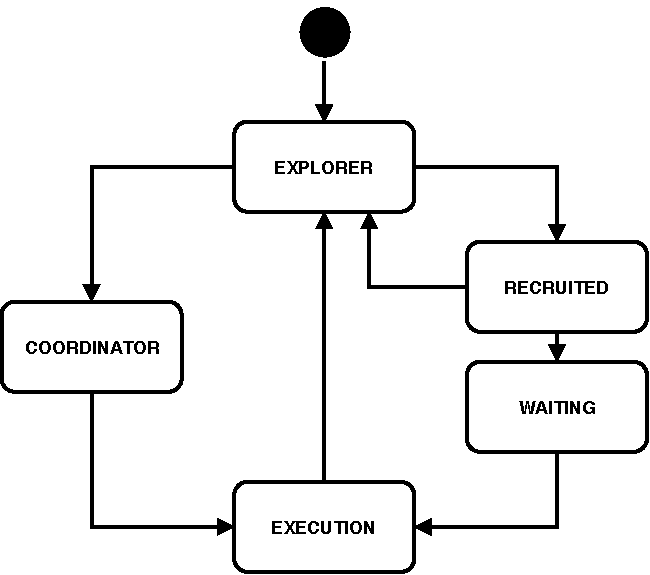
\includegraphics[width=0.3\paperwidth]{img/uav_states.pdf}}
    \end{center}
    \caption{Possibili stati di un drone}
    \label{uav_states}
\end{figure}

\section{Target}

I target si trovano in posizioni sconosciute a priori e devono essere scoperti e, se la missione lo prevede, eseguiti dai droni entro il loro tempo di autonomia.
Un target può essere, dunque, considerato come \textit{trovato} (found) quando un drone, equipaggiato con una tecnologia di sensing adeguata, si trova in una posizione tale da poterlo rilevare.
Un target è da considerare \textit{eseguito} (executed) nel momento in cui un subset dello sciame ha terminato la fase di esecuzione prevista dalla missione. \\
Alcuni esempi di target potrebbero essere:

\begin{itemize}
    \item mine antiuomo inesplose;
    \item discariche abusive;
    \item principi di incendi;
    \item \dots
\end{itemize}

\section{Ostacolo}

Un ostacolo è definito come un'entità statica all'interno dell'ambiente di simulazione, che non può essere attraversata dai droni.
Costruzioni e alberi rappresentano tipici esempi di ostacoli che possono trovarsi all'interno di un contesto applicativo.
Il numero, la forma e la dimensione degli ostacoli dipendono dalla quota di volo di un UAV: tipicamente, maggiore è la quota di volo e minore sarà il numero di ostacoli.

\section{Algoritmo bioispirato}

In questa sezione verranno esaminati alcuni punti chiave fondamentali che caratterizzano tipicamente gli algoritmi bioispirati, oggetto di comparazione all'interno dell'ambiente di simulazione.
Per semplificare la comprensione di tali meccanismi, verranno analizzati alcuni algoritmi presenti in letteratura che sono stati integrati all'interno del simulatore per un'analisi comparativa delle performance. 

\subsection{SciaDro}

Tale algoritmo è stato inizialmente integrato all'interno del simulatore Sciadro 3.1, pubblicamente rilasciato da Cimino et al. \cite{cimino2019adaptive}.
Nella sezione successiva verranno analizzati i meccanismi fondamentali di questa strategia:

\begin{itemize}
    \item \textit{Collision avoidance};
    \item \textit{Stigmergia};
    \item \textit{Flocking};
\end{itemize}

\subsubsection{Modulo di collision avoidance}

Tipicamente, come già anticipato, l’ambiente di esplorazione prevede la presenza di ostacoli. 
Il numero di droni utilizzati per il completamento della missione, inoltre, potrebbe essere elevato.
Di conseguenza, risulta strettamente necessario un meccanismo di collision avoidance al fine di rendere più realistica la simulazione. 
Il modulo di collision avoidance può essere suddiviso in due sottomoduli:

\begin{enumerate}
    \item \textit{Modulo di obstacle avoidance:} l’obiettivo principale di questo modulo software è quello di evitare le collisioni tra i droni e gli ostacoli presenti nell’ambiente di esplorazione. 
    In un contesto applicativo reale, questo meccanismo risulta strettamente necessario per ragioni di sicurezza e di costi;
    \item \textit{Modulo di overlap avoidance:} l’obiettivo di questo modulo è quello di evitare che si verifichino collisioni (o scontri) tra due o più droni in movimento. 
    Questa condizione deve essere sempre verificata, in particolare quando il numero di droni dello sciame aumenta.
\end{enumerate}

\subsubsection{Stigmergia}

La stigmergia è un meccanismo bio-ispirato usato da formiche, api ed altri insetti sociali, ad esempio durante l’attività di foraggiamento. 
La stigmergia è un meccanismo emergente, perché entità con limitate capacità computazionali possono organizzarsi in maniera distribuita e robusta.

L’elemento fondamentale della stigmergia è il feromone, ovvero una sostanza chimica in grado di attrarre altre entità nei luoghi in cui viene rilasciata. 
Il feromone ha una durata limitata nel tempo e dopo un certo periodo scompare a causa dell’evaporazione. 
Inoltre, un’entità attratta dal feromone è soggetta all’assuefazione olfattiva: dopo un certo tempo l’attrazione esercitata dal feromone perde il suo effetto.

Il meccanismo di stigmergia, così come descritto, è stato progettato, implementato e testato nel simulatore SciaDro. 
Lo scopo principale è quello di attrarre altre entità su un target di interesse comune, perché, in questo modo, altri target vicini possono essere facilmente scoperti.

Il feromone può essere anche repulsivo: invece di attrarre entità in un’area delimitata, respinge le entità vicine.

\subsubsection{Flocking}

Il flocking è il comportamento esibito quando un gruppo di uccelli, denominato flock, sta facendo attività di foraggiamento oppure è in volo. 
Il flocking è simile al comportamento di shoaling dei pesci, al comportamento di swarming degli insetti e ai comportamenti di altri animali sociali. 
La ragione principale per organizzare le entità in flocks sta nel fatto di raggrupparle per rendere più efficiente ed affidabile il processo di scoperta dei target. 
Infatti, un flock costituito da più droni ha un raggio di sensing più ampio rispetto al singolo drone. 
Il meccanismo di flocking può essere ulteriormente suddiviso in tre diversi sotto-meccanismi:

\begin{enumerate}
    \item \textit{Separazione:} il meccanismo di separazione ha l'obiettivo di distanziare i droni, sia per prevenire le collisioni, sia per avere dei flock più ampi così da incrementare la copertura dell'area di sensing;
    \item \textit{Allineamento:} il meccanismo di allineamento ha lo scopo di allineare il drone nella direzione media del flock al fine di seguire in modo più accurato gli altri droni della stessa flotta;
    \item \textit{Coesione:} questo meccanismo ha lo scopo di recuperare il flock e si attiva quando un’entità è “troppo lontana” dal resto dei compagni. 
    Tale lontananza rappresenta un parametro regolabile all'interno del simulatore.
\end{enumerate}

\subsubsection{Stati di un drone}

Nell'ultima versione dell'algoritmo è stato introdotto un meccanismo che prevede la modifica dello stato del drone, in accordo con determinati eventi che si scatenano durante lo svolgimento della missione.
Nel caso specifico, un drone può assumere uno dei seguenti stati, che verranno illustrati in dettaglio nella fase di progettazione:
\begin{itemize}
    \item \textit{Explorer};
    \item \textit{Waiting};
    \item \textit{Execution};
\end{itemize}

\subsection{Algortmi PAPER}

Gli autori in \cite{palmieri2017comparison} si sono concentrati sull'applicazione di diverse metaeuristiche di ispirazione biologica per il coordinamento di uno sciame che deve esplorare un'area sconosciuta al fine di trovare e gestire in modo cooperativo alcuni obiettivi distribuiti.
Di seguito verranno analizzate prima le metaeuristiche orientate all'esplorazione dell'area e successivamente quelle inerenti il coordinamento dello sciame per la gestione dei target identificati.

In questo caso, un agente può assumere tutti e 5 gli stati descritti nella sezione \ref{stati}.

\subsubsection{Esplorazione}

L'obiettivo della strategia di esplorazione è quello di visitare l'area d'interesse della missione in maniera efficiente, minimizzando la possibilità che gli attori visitino più volte una stessa area della regione.
A tal fine viene utilizzata una comunicazione basata sull'ambiente (\textit{stigmergia}) ed in particolare viene utilizzato un meccanismo feromonico repulsivo.
Durante l'esplorazione, il feromone viene depositato dal drone non appena si raggiunge la nuova cella. 
In questo modo, l'entità in movimento selezionerà la cella, appartenente al subset di celle immediatamente vicine alla posizione corrente, che presenta la traccia feromonica meno intensa.

L'uso dei feromoni è simile a quello del metodo \textit{Ant Colony Optimization}, ma a differenza delle formiche, in questo caso le celle più interessanti sono quelle senza feromoni o con il più piccolo valore di feromoni. 
Il feromone depositato si diffonde verso l'esterno, cella per cella, fino ad una certa distanza  e la quantità di feromone diminuisce con l'aumentare della distanza dal drone.


\subsubsection{Strategie di reclutamento}

Quando un bersaglio viene identificato, nel caso in cui la missione lo preveda, inizia un processo di reclutamento per poterlo gestire in modo cooperativo.
L'attore che ha trovato il target modifica il proprio stato in \textit{coordinator} ed inizia una comunicazione il cui fine è quello di richiamare altri droni all'obiettivo ed eseguire il task previsto dalla missione. 
Le metaeuristiche di reclutamento sono di tre diversi tipi:

\begin{enumerate}
    \item \textit{Firefly-based team strategy for robots recruitment (FTS-RR)}: tale metodo è basato sul \textit{Firefly Algorithm} sviluppato da Yang \cite{yang2009firefly}, \cite{yang2010firefly}. 
    L'obiettivo di questa strategia è quello di imitare il comportamento lampeggiante delle lucciole.
    Due importanti fattori sono la variazione dell’intensità luminosa e la formulazione del coefficiente di attrattività. 
    L’intensità della luce diminuisce con il quadrato della distanza, quindi le lucciole avranno visibilità limitata; inoltre l’attrattività è proporzionale alla luminosità quindi per ogni due lucciole lampeggianti la meno brillante si muoverà verso la più luminosa.
    \item \textit{Particle swarm optimization  for robots recruitment (PSO-RR)}: è una tecnica di ottimizzazione che utilizza una popolazione di agenti multipli \cite{eberhart1995particle}.
    Questa tecnica è stata ispirata dal movimento degli uccelli e dalle loro interazioni con i vicini nello stormo.
    \item \textit{Artificial bee colony algorithm  for robots recruitment (ABC-RR)}: questo approccio è basato sull'algoritmo ABC sviluppato da Karaboga et al. in \cite{karaboga2009comparative}.
    Esso segue il comportamento delle api in cerca di una fonte di nutrimento di qualita. Le api possono essere classificate in tre gruppi: \textit{employed bees}, \textit{onlooker bees} e \textit{scout bees}. 
    Le api \textit{employed} sfruttano le posizioni degli accumuli di cibo, mentre le api \textit{onlooker} sono in attesa di informazioni dalle api \textit{employed} sulla quantità di nettare di tali accumuli. 
    Le api \textit{onlooker} prenderanno la decisione di scegliere una fonte alimentare sulla base di queste informazioni.
    Una fonte alimentare di qualità superiore avrà una maggiore probabilità di essere selezionata dalle api \textit{onlooker}. Infine, le api \textit{scout} trovano nuove fonti di nutrimento nell'ambiente.
\end{enumerate}
\chapter{Progettazione}

Nella fase di progettazione, si sono fatte alcune assunzioni sull'ambiente, sul drone e sulle altre entità coinvolte durante la fase di simulazione.
In particolare, tali assunzioni riguardano le caratteristiche principali dell'ambiente e delle entità in esso coinvolte.

\section{Progettazione dell'ambiente}

L'ambiente che viene preso in esame dipende dallo scenario considerato per la simulazione della missione.
Esso rappresenta un'area bidimensionale strutturata e limitata, in cui lo spazio ed il tempo risultano entrambi discretizzati.

Lo spazio è simulato attraverso una griglia di \textit{NxM} celle quadrate, dette \textit{patch}, di lato \textit{S}. 
Il tempo è discretizzato in una sequenza di intervalli temporali di durata \textit{T} detti \textit{tick} definiti come:
\begin{equation*}
    t_0 + T, t_0 + 2T, \dots, t_0 + NT
\end{equation*}

L'ambiente simulato contiene i seguenti elementi: 
\begin{itemize}
    \item \textit{Droni};
    \item \textit{Target};
    \item \textit{Ostacoli};
    \item \textit{Feromoni digitali};
\end{itemize}

La figura \ref{elementi_ambiente} mostra una rappresentazione semplificata dell'ambiente di simulazione con gli elementi sopra descritti.

Nell'ambiente, un singolo UAV è rappresentato da un disco con un punta di freccia interna. 
La punta indica la direzione del drone. 
Ostacoli e target, solitamente, coprono diverse celle.
In figura, ogni cella in cui è presente un ostacolo è nera, mentre ogni cella-target è colorata. 
Come abbiamo già precedentemente accennato, un target può assumere diversi stati: in questo caso un target \textit{not found} è rappresentato da una cella rossa, un target \textit{found} da una cella verde e con una cella gialla, infine, un target \textit{executed}.
L'intensità del colore di bersaglio, quando applicabile (ad esempio, fuoco, gas, ecc.), rappresenta la quantità/presenza del target. 
Infine, una traccia feromonica è indicata da un gruppo di cellule grigie, dove la scala di grigio varia in base all'intensità dei feromoni.

\begin{figure}[H] 
    \captionsetup{justification=centering, margin=2cm, font=footnotesize}
    \begin{center}
    \makebox[\textwidth]{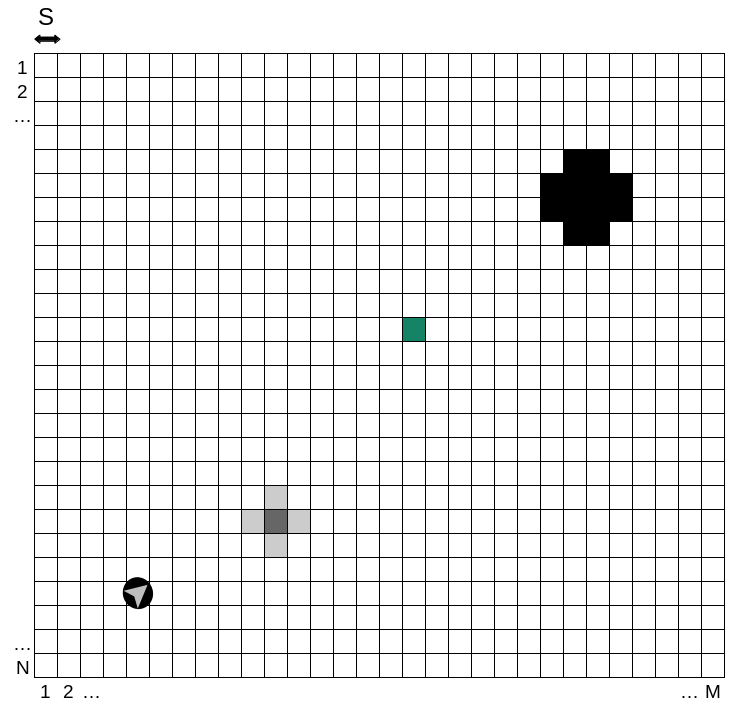
\includegraphics[width=0.4\paperwidth]{img/elementi_ambiente.png}}
    \end{center}
    \caption[short]{Definizione dell'ambiente simulato: (da sinistra a destra) drone, feromone, target ed ostacolo.}
    \label{elementi_ambiente}
\end{figure}

Si assumano, per semplicità i seguenti valori:
\begin{itemize}
    \item S = 1 metro;
    \item T = 1 secondo; 
\end{itemize}

I valori sopra riportati, naturalmente, possono variare in base alla missione ed allo scenario in cui essa si svolge.
In questo caso, l'assunzione è necessaria per una conversione immediata da metri a numero di patch e da secondi a tick.

Supponendo di avere una patch di lato \textit{S} diverso da un metro, può essere sfruttata la seguente formula di conversione, per determinare il numero di patch a cui corrisponde un metro:

\begin{equation}
    \label{m_patches}
    1 \; m = \frac{1}{S} \; patches
\end{equation}

Allo stesso modo, si può determinare a quanti tick corrisponde un secondo:

\begin{equation}
    \label{sec_ticks}
    1 \; s = \frac{1}{T} \; ticks
\end{equation}

Dalle relazioni \ref{m_patches} e \ref{sec_ticks} è possibile determinare la formula di conversione da \textit{m/s} a \textit{patches/tick}:

\begin{equation*}
    1 \; m/s = (\frac{1}{S})(\frac{1}{T}) \; patches/tick 
\end{equation*}

Ad ogni tick, il drone effettua rilevamenti di ostacoli, target e feromoni vicini alla sua posizione ed esegue regole comportamentali precise.
Lo sciame di droni si muove separatamente, organizzato in diversi flock.

Il blocco fondamentale dello spazio discretizzato simulato è rappresentato dalla cella.
Ogni cella (denominata anche patch) ha delle coordinate \textit{x-y} nello spazio bidimensionale e può contenere un target o un ostacolo.
Una caratteristica fondamentale del simulatore è la possibilità di prenotare una patch: tale strategia, infatti, è pensata nel caso in cui è previsto un meccanismo di \textit{collision avoidance}, come nel caso dell'algoritmo SCIADRO.

Per illustrare la struttura di un oggetto \textit{patch}, consideriamo la cella come una classe.
Nella figura \ref{classe_patch} è possibile osservare tale struttura.

\begin{figure}[H] 
    \captionsetup{justification=centering, margin=2cm, font=footnotesize}
    \begin{center}
    \makebox[\textwidth]{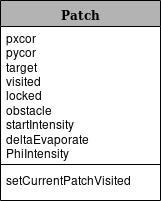
\includegraphics[width=0.2\paperwidth]{img/classe_patch.png}}
    \end{center}
    \caption[short]{Struttura della classe Patch.}
    \label{classe_patch}
\end{figure}

\section{Elemento ostacolo}

Un ostacolo è un elemento che ostruisce il passaggio di un UAV. 
Esso ha una posizione statica e occupa una cella all’interno dell’ambiente di esplorazione. 
L’ostacolo non può essere attraversato dal drone e rappresenta la base per modellare diversi tipi di strutture come, ad esempio, alberi, costruzioni, ecc.

\section {Elemento target}

Un target è un elemento collocato, all'istante \textit{t}, in una determinata posizione dell’ambiente di simulazione sconosciuta ai droni. 
La struttura di un target dipende da cosa si vuole modellare, in accordo con il task della missione:

\begin{itemize}
    \item \textit{Rilevamento di sostanze}, come un gas o un liquido tossico: in questo caso gli elementi sono modellati attraverso una distribuzione gaussiana di target, con media in corrispondenza della sorgente;
    \item \textit{Identificazione di oggetti}, come ad esempio mine anti-uomo: in questo caso il target è modellato come una singola cella;
    \item \dots
\end{itemize}

Lo stato di un target è identificato dalla variabile \textbf{target.state}, che può assumere i seguenti valori:

\begin{itemize}
    \item \textit{Found};
    \item \textit{Not found};
    \item \textit{Executed}.
\end{itemize}

\begin{figure}[H] 
    \captionsetup{justification=centering, margin=2cm, font=footnotesize}
    \begin{center}
    \makebox[\textwidth]{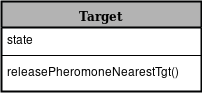
\includegraphics[width=0.2\paperwidth]{img/classe_target.png}}
    \end{center}
    \caption[short]{Struttura della classe Target.}
    \label{classe_target}
\end{figure}

\section {Elemento UAV}

L'UAV è l'elemento in grado di muoversi in modo continuo all’interno dello spazio bidimensionale di ricerca con l’obiettivo principale di scoprire nuovi target. 
Inoltre, il drone deve evitare di scontrarsi con gli ostacoli o con altri droni e, insieme a loro, deve coordinarsi e completare il processo di scoperta dei target entro il tempo di autonomia, usando meccanismi di comunicazione diretta o indiretta, in base all’algoritmo integrato nel simulatore. 

Gli scontri e le collisioni con altri droni e con gli ostacoli sono, naturalmente, simulati. 
Per questo motivo, a partire dalla fase di progettazione, questi eventi possono essere denominati “sovrapposizioni tra droni e droni” e “sovrapposizioni tra droni e ostacoli”, rispettivamente. 
Si deve notare che il sensing potrebbe essere influenzato dalla velocità del drone. 
Esiste una velocità massima per cui la performance della tecnologia di sensing non risulta influenzata dalla velocità del drone: tale velocità è denominata velocità di crociera e risulta minore della velocità massima.

\section {Algoritmo bioispirato}

Alcune caratteristiche degli elementi presenti nel simulatore, come la struttura del drone o del feromone digitale, dipendono dall'algoritmo integrato all'interno dell'ambiente di simulazione.
Nella sezione successiva ci soffermeremo sulle metaeuristiche della strategia \textit{Sciadro}.
Successivamente, invece, prenderemo in esame gli elementi utilizzati nel gruppo di algoritmi analizzati precedentemente: \textit{FTS}, \textit{PSO} e \textit{ABC}.

\subsection{SciaDro}

In questa sezione entreremo nel dettaglio della progettazione dei vari elementi introdotti nel capitolo \ref{analisi} (\textit{Analisi}), quali il drone ed i vari meccanismi di flocking, collision avoidance e stigmergia.

\subsubsection{Progettazione del drone}

Il drone può essere modellato come un cerchio in movimento nello spazio bidimensionale. 
I parametri associati al drone dipendono dalle sue caratteristiche fisiche e architetturali. 
Lo stato del drone è caratterizzato da:

\begin{itemize}
    \item Posizione nell’ambiente (\textbf{drone.x} e \textbf{drone.y});
    \item Numero di droni vicini nello sciame (\textbf{drone.flockmates});
    \item Velocità di crociera (\textbf{drone.cruisingSpeed});
    \item Velocità corrente (\textbf{drone.speed});
    \item Direzione corrente (\textbf{drone.heading});
    \item Velocità angolare corrente (\textbf{drone.angularSpeed});
    \item Autonomia (\textbf{drone.endurance}).
\end{itemize}
Il drone esegue azioni al fine di:

\begin{enumerate}
    \item Evitare ostacoli
    \begin{itemize}
        \item Collision avoidance
    \end{itemize}
    \item Coordinarsi con gli altri droni attraverso il meccanismo di flocking
    \begin{itemize}
        \item Separate
        \item Align
        \item Cohere
    \end{itemize}
    \item Rilasciare il feromone
    \item Muoversi nell’ambiente per ricercare i targets
    \begin{itemize}
        \item Movement
        \item Accelerate
        \item Decelerate
    \end{itemize}
\end{enumerate}

Al fine di rilevare il target, è stato necessario inserire un codice di sensing. L’area del cono di sensing dipende prevalentemente dal tipo di sensore. 

Per le ragioni sopra menzionate, tutti questi parametri devono essere fissati prima di avviare la simulazione.

\begin{figure}[H] 
    \captionsetup{justification=centering, margin=2cm, font=footnotesize}
    \begin{center}
    \makebox[\textwidth]{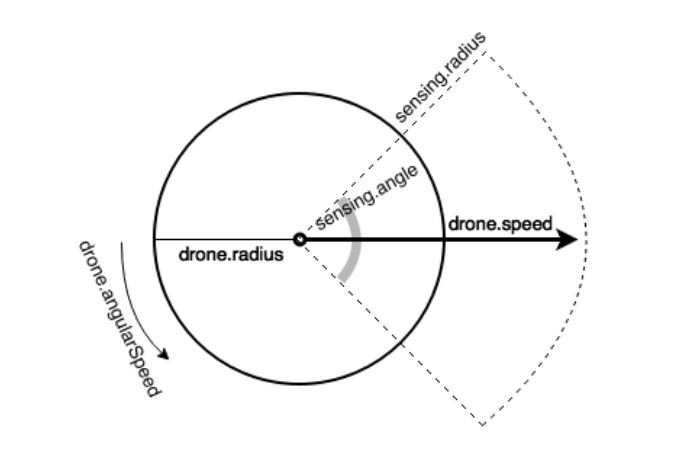
\includegraphics[width=0.4\paperwidth]{img/modello_parametrico_drone.png}}
    \end{center}
    \caption[short]{Modello parametrico del drone.}
    \label{modello_drone}
\end{figure}

La seguente tabella riassume i parametri strutturali che caratterizzano il drone.
\begin{table}[H]
    \centering
    \begin{tabular}{|l|l|c|}
    \hline
    \textbf{Parametro}       & \textbf{Definizione}       & \textbf{Unità di misura}   \\ \hline
    drone.radius             & Raggio fisico              & (m)                        \\ \hline
    sensing.radius           & Raggio di sensing          & (m)                        \\ \hline
    sensing.angle            & Angolo di sensing          & (gradi)                    \\ \hline
    drone.cruisingSpeed      & Velocità di crociera       & (m/s)                      \\ \hline
    drone.speedMax           & Velocità massima           & (m/s)                      \\ \hline
    drone.speed              & Velocità corrente          & (m/s)                      \\ \hline
    drone.acceleration       & Accelerazione              & (m/s\textsuperscript{2})   \\ \hline
    drone.deceleration       & Decelerazione              & (m/s\textsuperscript{2})   \\ \hline
    drone.endurance          & Autonomia                  & (minuti)                   \\ \hline
    drone.heading            & Direzione corrente         & (gradi)                    \\ \hline
    drone.accelerationAng    & Accelerazione angolare     & (rad/s\textsuperscript{2}) \\ \hline
    drone.decelerationAng    & Decelerazione angolare     & (rad/s\textsuperscript{2}) \\ \hline
    drone.velocityAngularMax & Velocità angolare massima  & (rad/s\textsuperscript{2}) \\ \hline
    drone.angularSpeed       & Velocità angolare corrente & (rad/s\textsuperscript{2}) \\ \hline
    \end{tabular}
    \caption{Parametri strutturali del drone.}
\end{table}

Ad ogni ciclo di aggiornamento, il drone assume una posizione specifica nello spazio di ricerca, descritta da una coppia di coordinate.
Esso può essere equipaggiato con uno o più sensori e può muoversi sia in modo longitudinale che rotazionale.
Il drone, inoltre, è anche in grado di rilevare i target e di rilasciare impronte di feromone per la comunicazione indiretta con gli altri UAV.

\begin{figure}[H] 
    \captionsetup{justification=centering, margin=2cm, font=footnotesize}
    \begin{center}
    \makebox[\textwidth]{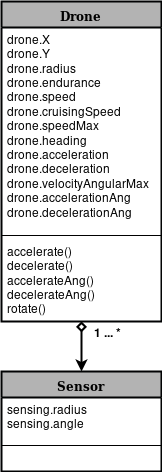
\includegraphics[width=0.2\paperwidth]{img/classe_drone.png}}
    \end{center}
    \caption[short]{Struttura della classe Drone.}
    \label{classe_drone}
\end{figure}

\subsubsection{Progettazione del flocking}

Di seguito si illustra la progettazione del meccanismo di flocking descritto nella fase di analisi. 
Il drone distingue tre diverse aree di prossimità: l’area di separazione (\textit{separate}), l’area di allineamento (\textit{align}) e l’area di coesione (\textit{cohere}). 
Ciascuna di tali aree ha uno specifico raggio ed è associata ad uno specifico comportamento del drone.
Le tre aree di prossimità hanno in comune l’angolo \textbf{drone.flocking.angle}.

\begin{figure}[H] 
    \captionsetup{justification=centering, margin=2cm, font=footnotesize}
    \begin{center}
    \makebox[\textwidth]{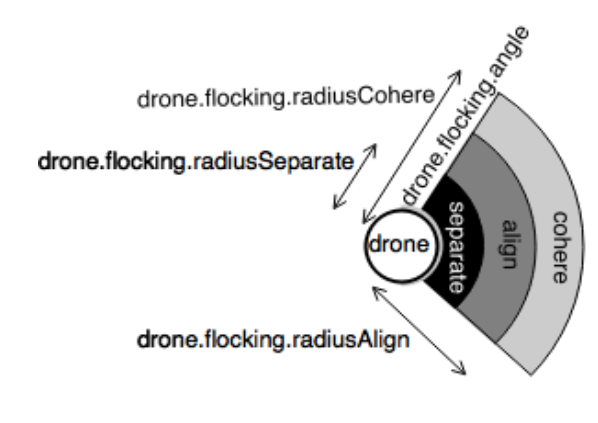
\includegraphics[width=0.4\paperwidth]{img/aree_flocking.png}}
    \end{center}
    \caption[short]{Aree del meccanismo di flocking.}
    \label{aree_flocking}
\end{figure}

I parametri illustrati nella figura \ref{aree_flocking}, sono analizzati in dettaglio nella seguente tabella.
\begin{table}[H]
    \centering
    \resizebox{\textwidth}{!}{%
    \begin{tabular}{|l|l|c|}
    \hline
    \textbf{Parametro}             & \textbf{Definizione}                                                                    & \textbf{Unità di misura} \\ \hline
    drone.flocking.angle           & Angolo di visione del flock                                                             & (gradi)                  \\ \hline
    drone.flocking.radiusCohere    & Raggio di coesione $\in$ [drone.flocking.radiusAlign, +$\infty$)                            & (m)                      \\ \hline
    drone.flocking.maxCohereTurn   & Angolo di rotazione massimo nel meccanismo di coesione                                  & (gradi)                  \\ \hline
    drone.flocking.radiusAlign     &\begin{tabular}[c]{@{}l@{}}Raggio di allineamento $\in$ [drone.flocking.radiusSeparate, \\ drone.flocking.radiusCohere]\end{tabular} & (m)                      \\ \hline
    drone.flocking.maxAlignTurn    & Angolo di rotazione massimo nel meccanismo di allineamento                              & (gradi)                  \\ \hline
    drone.flocking.radiusSeparate  & Raggio di separazione $\in$ [drone.collisionVision, +$\infty$)                              & (m)                      \\ \hline
    drone.flocking.maxSeparateTurn & Angolo di rotazione massimo nel meccanismo di separazione                               & (gradi)                  \\ \hline
    drone.flocking.wiggleVar       & Numero casuale [0,N]                                                                    & (adimensionale)          \\ \hline
    \end{tabular}%
    }
    \caption{Parametri strutturali del flocking.}
    \label{tabella_flocking}
\end{table}

\paragraph{Comportamento separate:} se un drone si trova all'interno dell'area identificata dal raggio \textbf{drone.flocking.radiusSeparate}, allora viene attivato il meccanismo di separazione, ovvero una rotazione che porta il drone a separarsi dal resto del flock.
Tale rotazione è limitata all'angolo \textbf{drone.flocking.maxSeparateTurn}.

\begin{figure}[H] 
    \captionsetup{justification=centering, margin=2cm, font=footnotesize}
    \begin{center}
    \makebox[\textwidth]{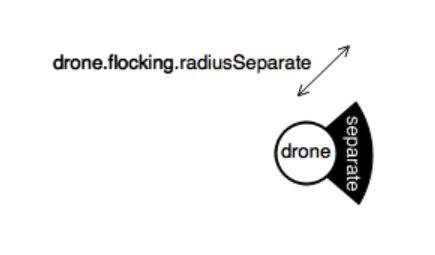
\includegraphics[width=0.4\paperwidth]{img/separate.png}}
    \end{center}
    \caption[short]{Area di riferimento per il comportamento \textit{Separate}.}
    \label{separate}
\end{figure}

\paragraph{Comportamento aling:} il drone verifica la presenza di altri droni nell'area di align e ruota di un angolo \textbf{drone.flocking.alignAngle}, più un angolo casuale \textbf{drone.flocking.wiggleVar}, al fine di allinearsi al resto del flock.
Tale rotazione è limitata all'angolo  \textbf{drone.flocking.maxAlignTurn}.

\begin{figure}[H] 
    \captionsetup{justification=centering, margin=2cm, font=footnotesize}
    \begin{center}
    \makebox[\textwidth]{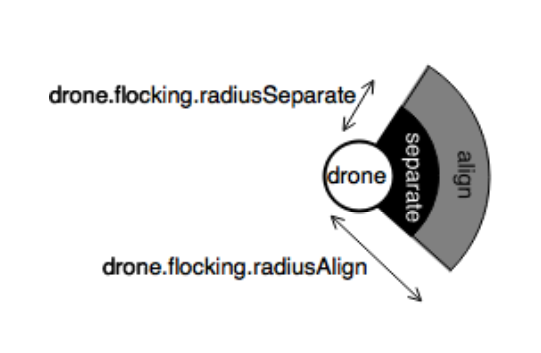
\includegraphics[width=0.4\paperwidth]{img/align.png}}
    \end{center}
    \caption[short]{Area di riferimento per il comportamento \textit{Align}.}
    \label{align}
\end{figure}

\paragraph{Comportamento cohere:} il drone calcola il baricentro dei compagni di flock presenti nell'area di cohere, il cui raggio è \textbf{drone.flocking.radiusCohere}, e ruota in quella direzione.
La massima rotazione permessa è un angolo pari a \textbf{drone.flocking.maxCohereTurn}, più una quantità \textbf{drone.flocking.wiggleVar} casuale.

\begin{figure}[H] 
    \captionsetup{justification=centering, margin=2cm, font=footnotesize}
    \begin{center}
    \makebox[\textwidth]{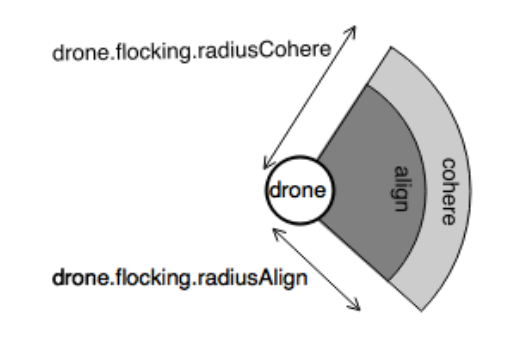
\includegraphics[width=0.4\paperwidth]{img/cohere.png}}
    \end{center}
    \caption[short]{Area di riferimento per il comportamento \textit{Cohere}.}
    \label{cohere}
\end{figure}

\paragraph{Algoritmo di flocking:} come già ampiamente illustrato, il meccanismo di flocking è costituito da tre sottomeccanismi a priorità decrescente:
\begin{itemize}
    \item Separate;
    \item Align;
    \item Cohere.
\end{itemize}

Ad ogni ciclo di aggiornamento (\textit{tick}), può essere eseguito solo uno di questi comportamenti.
La figura \ref{activity_flocking} rappresenta il diagramma di attività dell'algoritmo di flocking, in cui viene omessa, per semplicità, la variabile casuale \textit{wiggleVar}.

\begin{figure}[H] 
    \captionsetup{justification=centering, margin=2cm, font=footnotesize}
    \begin{center}
    \makebox[\textwidth]{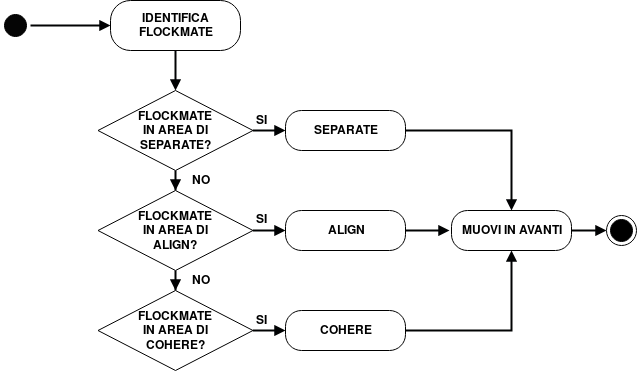
\includegraphics[width=0.5\paperwidth]{img/activity_flocking.png}}
    \end{center}
    \caption[short]{Diagramma di attività dell'algoritmo di flocking.}
    \label{activity_flocking}
\end{figure}

Tutti i parametri di flocking sono fissati prima di avviare la simulazione ed influenzano il movimento del drone e dunque il comportamento del flock.

\begin{figure}[H] 
    \captionsetup{justification=centering, margin=2cm, font=footnotesize}
    \begin{center}
    \makebox[\textwidth]{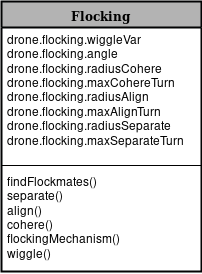
\includegraphics[width=0.2\paperwidth]{img/classe_flocking.png}}
    \end{center}
    \caption[short]{Diagramma della classe Flocking.}
    \label{classe_flocking}
\end{figure}

\subsubsection{Progettazione del meccanismo di collision avoidance}

Il meccanismo di collision avoidance risulta indispensabile, considerato che i droni non devono scontrarsi tra loro o con gli ostacoli presenti all'interno dell'area simulata.
Tale meccanismo può essere suddiviso in due sottomeccanismi:

\begin{itemize}
    \item \textit{Obstacle avoidance}: permette di evitare collisioni tra un drone ed un ostacolo;
    \item \textit{Overlapping avoidance}: permette di evitare collisioni tra droni.
\end{itemize}

\paragraph{Modello di obstacle avoidance:} il modello segue una semplice regola: trovare il gap tra ostacoli che comporta la minima rotazione del drone verso il gap stesso. 
La semplicità di questa regola è dovuta al fatto che il drone ha un tempo limitato per riconoscere l’ostacolo, trovare il gap e ruotare verso la sua direzione.

In un contesto reale, il drone può trasportare un array di sensori ad infrarossi in grado di riconoscere le distanze e gli angoli degli ostacoli vicini. 
L’attività di riconoscimento di un ostacolo è modellata così come fatto per il sensing: un cono con un certo angolo e un certo raggio. 
Il drone, dopo aver calcolato le distanze e gli angoli degli ostacoli vicini, ricerca il gap che comporta la minore rotazione rispetto alla direzione corrente.

A causa della grande varietà di ostacoli che si possono trovare nei diversi contesti applicativi, sia la dimensione del gap che il raggio e l’angolo di visione degli ostacoli risultano configurabili. 
Durante la simulazione, questi parametri influenzano il comportamento del drone, perché l’algoritmo di obstacle avoidance dipende dal loro valore.

\begin{table}[H]
    \centering
    \resizebox{\textwidth}{!}{%
    \begin{tabular}{|l|l|c|}
    \hline
    \textbf{Parametro}             & \textbf{Definizione}                                                                                                                                               & \textbf{Unità di misura} \\ \hline
    drone.collision.gapAngle       &\begin{tabular}[c]{@{}l@{}}Minimo angolo che permette al drone di passare attraverso \\ il varco tra due ostacoli $\in$ [0, drone.sight.angleMax]\end{tabular}   & (gradi)                  \\ \hline
    drone.collision.vision         & Raggio di visibilità degli ostacoli                                                                                    & (m)                      \\ \hline
    drone.sight.angleMax           & Massimo angolo di visibilità degli ostacoli                                                                            & (gradi)                  \\ \hline
    \end{tabular}%
    }
    \caption{Parametri strutturali del meccanismo di obstacle avoidance.}
    \label{tabella_obstacle_avoidance}
\end{table}

\subsubsection{Progettazione dell'impronta di feromone attrattivo}

\subsection{Algortmi PAPER}
\chapter{Ottimizzazione parametrica e valutazione delle performance}

L'obiettivo dell'ambiente di simulazione è quello di valutare le performance dell'algoritmo integrato per stabilire la migliore configurazione dei parametri in un dato contesto applicativo.
Data l'eterogeneità delle missioni, infatti, non è possibile stabilire una configurazione di parametri che sia ottimale per tutti gli scenari.

Come abbiamo già più volte sottolineato nei capitoli precedenti, l'obiettivo di uno sciame è quello di identificare, entro il tempo di autonomia, i target presenti nell'area di esplorazione.
Una valutazione delle performance, di conseguenza, può essere eseguita in considerazione del tempo impiegato per il rilevamento (o per l'esecuzione, se la missione lo richiede) di almeno il $95\%$ dei target (\textit{discovering time}).
Una migliore configurazione dei parametri in ingresso, in relazione alla strategia di coordinamento adottata, comporterà un \textit{discovering time} inferiore.

Un altro parametro per la valutazione delle performance è rappresentato dal numero di collisioni, che risulta importante per due ragioni fondamentali:
\begin{enumerate}
    \item \textit{Costi:} in un contesto reale, la perdita di un drone può avere un impatto economico piò o meno rilevante a seconda del tipo di UAV;
    \item \textit{Rischi:} la collisioni di un drone può avere ripercussioni anche sull'incolumità di persone o cose.
\end{enumerate}

Al fine di ottenere un risultato significativo da un punto di vista statistico, la valutazione delle performance di un insieme di parametri viene  valutata come media su più esecuzioni indipendenti del simulatore.

\section{Ottimizzazione basata su \\\textit{Differential Evolution}}

L’algoritmo \textit{Differential Evolution} è uno strumento software in grado di trovare la configurazione ottimale dei parametri per un problema caratterizzato da una specifica complessità. 
Risulta importante sottolineare che l’algoritmo \textit{Differential Evolution} non garantisce la soluzione ottima del problema, ma una soluzione ottimale, ovvero una soluzione “vicina” a quella ottima. 

Nel caso in oggetto, lo strumento \textit{Differential Evolution} è utilizzato per configurare i parametri relativi al coordinamento previsto dall’algoritmo integrato nel simulatore. 
L’obiettivo principale del simulatore, infatti, è quello di valutare l’impatto dei meccanismi di coordinamento di uno sciame di UAV sui diversi scenari applicativi. 

L’algoritmo \textit{DE} ricerca il valore ottimale per ciascun parametro di configurazione all’interno di un intervallo definito a priori. 
Gli estremi di tale intervallo devono essere scelti in modo accurato in relazione alle caratteristiche del contesto applicativo e alle specifiche reali dei droni e dei sensori di rilevamento.

\subsection{Funzionamento dell'algoritmo \textit{Differential Evolution}}

Il Differential Evolution è un algoritmo evolutivo capace di gestire correttamente funzioni non differenziabili e non lineari. 
La ricerca del valore ottimo inizia con una popolazione generata in modo casuale, dove i valori assunti da ciascun elemento sono vincolati ad intervalli scelti a priori. 
Ad ogni iterazione, viene calcolato il risultato di una funzione obiettivo, detta \textit{fitness function}, sui vettori di parametri della generazione corrente.
L'obiettivo è quello di minimizzare il risultato di questa funzione operando con i meccanismi di evoluzione differenziale.

Come molti algoritmi che rientrano in questa categoria, opera con tre operazioni fondamentali: mutazione, crossover, selezione. 
Lo spazio delle soluzioni viene esplorato attraverso dei vettori di parametri generati per differenza; questo comportamento si individua nell’operazione di mutazione. Questa rappresenta la maggior differenza con gli algoritmi genetici, che utilizzano l’operazione di crossover (rimescolamento di geni) come primo meccanismo di ricerca. 

Il Differential Evolution utilizza delle differenze pesate fra i vettori delle soluzioni al fine di perturbare la popolazione e non richiede, inoltre, la codifica binaria dei membri della popolazione.

\begin{figure}[H] 
    \captionsetup{justification=centering, margin=2cm, font=footnotesize}
    \begin{center}
    \makebox[\textwidth]{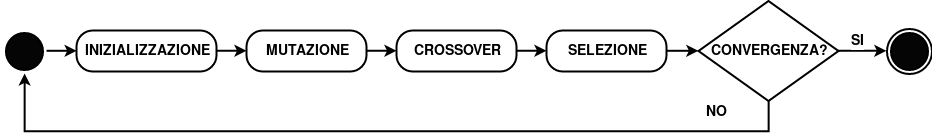
\includegraphics[width=0.6\paperwidth]{img/de_steps.png}}
    \end{center}
    \caption{Algoritmo Differential Evolution step-by-step.}
    \label{de_steps}
\end{figure}

Di seguito, si riporta lo pseudocodice del \textit{Differential Evolution}.
Nei paragrafi successivi, invece, verranno descritte nel dettaglio le tre operazioni fondamentali sopra introdotte.

\begin{figure}[H]
    \centering
    \begin{minipage}{\linewidth}
    \begin{algorithm}[H]
    \SetAlgoLined
        \Begin {
            generate randomly an initial population of solutions \;
            compute the fitness function of the initial population \;
            \While {stop condition !satisfied}{
                \For {each parent}{
                    select three solutions at random \;
                    create one offspring using the DE operators \;
                }
                \For {each member of the next generation}{
                    \If {offspring(x) is more fit than parent(x)}{
                        parent(x) is replaced \;
                    }
                }
            }
        }
    \end{algorithm}
    \end{minipage}
    \caption{Pseudocodice Differential Evolution.}
\end{figure}

\subsubsection{Mutazione}

Il meccanismo di mutazione è utilizzato per produrre una popolazione di $NP$ vettori, dove $NP$ rappresenta il numero di individui nella popolazione.
In particolare, questa operazione genera un nuovo vettore mutante, aggiungendo una frazione della differenza tra due vettori, selezionati casualmente, ad un terzo.

L'implementazione elementare di questa operazione è descritta dall'espressione di seguito riportata:
\begin{equation*}
    v_{i} = x_{r_{0}} \; + \; F(x_{r_{1}} - x_{r_{2}})
\end{equation*}
Dove:
\begin{itemize}
    \item $v_{i}$ è il nuovo vettore mutante;
    \item I termini $x_{r_i}$, con $i = 0,1,2$, rappresentano i tre vettori selezionati casualmente tra quelli disponibili;
    \item La funzione $F \in (0,1+)$ regola il tasso di evoluzione della popolazione.
\end{itemize}

\subsubsection{Crossover}

Questa operazione produce i vettori da testare a partire dai vettori di parametri.
In particolare, viene incrociato ogni vettore della popolazione attuale con un vettore mutante prodotto dall'operazione precedente.

L'espressione per descrivere la fase di crossover è la seguente:
\begin{equation*}
    u_{i} = \begin{cases}
        v_{i,j} \; , \text{se } rand_{j}(0,1) \leq Cr \\
        u_{i,j} \; , \text{altrimenti} 
    \end{cases}
\end{equation*}

In altre parole, il nuovo individuo viene generato scegliendo tra il vettore mutante e quello corrente, con una probabilità $Cr$, detta \textit{probabilità di crossover}.
Tale probabilità è un parametro definito dall'utente.

\subsubsection{Selezione}

Se il vettore della soluzione in uso, $u_{i}$, ottiene un valore della funzione obiettivo minore o uguale rispetto alla soluzione candidata migliore, questa viene sostituita dal vettore $u_{i}$ nella generazione successiva.
\begin{equation*}
    x_{i,g+1} = \begin{cases}
        u_{i,g} \; , \text{se } f(u_{i,g}) \leq f(x_{i,g}) \\
        x_{i,g} \; , \text{altrimenti} 
    \end{cases}
\end{equation*}

\subsection{Implementazione software \textit{Differential Evolution}}

Al fine di ottimizzare i parametri di simulazione, è stato implementato un modulo software di evoluzione differenziale, chiamato \textit{Differential\_evolution\_bridge}.
Attraverso tale modulo, è possibile calcolare la funzione obiettivo tramite l'esecuzione di una simulazione con il vettore di parametri passato in input alla funzione.

La \textit{fitness function} è calcolata come segue:
\begin{equation*}
    fitness(x) = \#ticks[simulation(x)]
\end{equation*}
Dove:
\begin{itemize}
    \item $x$ rappresenta l'individuo della generazione attuale, ovvero il vettore di parametri dato in input alla simulazione;
    \item $\#ticks$ rappresenta il numero di iterazioni necessarie al rilevamento del $95\%$ di target;
    \item $simulation(x)$ indica l'esecuzione di una sessione simulativa con i parametri di $x$.
\end{itemize}

Differential evolution bridge utilizza, come implementazione software dell’evoluzione differenziale, la procedura presente nella libreria Python Scipy.Optimize, denominata \textit{differential\_evolution}.
Il modello algoritmico seguito è quello offerto da Kenneth Price e Rainer Storn in \cite{storn1997differential}, implementato secondo la libreria Scipy \cite{jones2014scipy}.
\chapter{Implementazione e prove sperimentali}

In questo capitolo verranno presentate le caratteristiche tecnologiche dei veicoli utilizzati nella fase sperimentale, le proprietà fisiche di ogni scenario modellato e le varie misure di qualità.

Per ogni scenario verrà illustrata la complessità ambientale, insieme alla rappresentazione reale ed al modello della relativa mappa, per comprendere le caratteristiche morfologiche dell'area e la strattura degli ostacoli presenti.
Verranno, inoltre, analizzate le informazioni relative ai parametri utilizzati nella fase di ottimizzazione e adattamento delle metaeuristiche alla missione.

Nel caso dello scenario \textit{Illegal Dump} sono state adattate entrambe le strategie di esplorazione analizzate nei capitoli precedenti e la strategia di reclutamento di SFE-RR, per dimostrare la possibilità di adattare strategie con diversi livelli di astrazione.
Nel caso degli scenari \textit{Rural Mine} e \textit{Urban Mine}, invece, l'adattamento interessa solo la strategia di esplorazione di SFE-RR, al fine di comparare le performance del simulatore, ed in particolare del modulo di ottimizzazione parametrica, con quelle ottenute in \cite{cimino2019adaptive}, nel quale l'ottimizzazione parametrica è implementata in Matlab.
A tal proposito, nelle sezioni dedicate alla comparazione di questi approcci, chiameremo \textit{SFE-RR1} il simulatore analizzato in questo documento, a voler indicare che il numero minimo di droni per eseguire il target è 1, e con \textit{SFE} l'ambiente di simulazione analizzato in \cite{cimino2019adaptive}.
In questo modo la comparazione tra le due strategie è consistente.
In generale, la notazione\textit{SFE-RRx} indica che il numero minimo di droni per l'esecuzione del target è \textit{x}.

Infine, i risultati sperimentali verranno presentati alla fine di ogni scenario ed alla fine del capitolo per un'analisi comparativa con i risultati già presenti in letteratura.
Per una presentazione consistente delle performance sono stati calcolati gli intervalli di confidenza del 95\% per il valore medio delle performance risultanti da ogni esperimento.
Per tale ragione è stato necessario verificare, attraverso un \textit{QQ-Plot}, che i risultati di ogni esecuzione dell'algoritmo di DE seguissero una distribuzione gaussiana.

\section{Specifiche tecniche del drone}

Le caratteristiche ambientali dei vari scenari sono state prese in considerazione per le specifiche tecniche degli UAV disponibili in commercio. 
La tecnologia selezionata per modellare gli agenti responasbili del completamento della missione è la seguente:
\begin{itemize}
    \item \textit{Modello drone:} Dji Matrice M200
    \item \textit{Sensore di rilevamento:} Dji Zenmuse XT2 (Visual + Thermal Camera) 
\end{itemize}
Tale tecnologia è stata adottata sulla base delle conoscenze e delle competenze acquisite in diversi progetti che utilizzano la tecnologia UAV per il monitoraggio e la sorveglianza ambientale. 
In particolare, la tecnologia di rilevamento proposta, si basa su \cite{persechino2010aerospace} e \cite{lega2012using};

\begin{figure}[H] 
    \captionsetup{justification=centering, margin=2cm, font=footnotesize}
    \begin{center}
    \makebox[\textwidth]{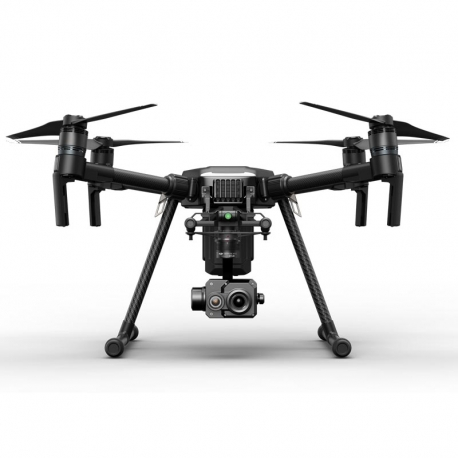
\includegraphics[width=0.4\paperwidth]{img/dji_matrice_sensore.jpg}}
    \end{center}
    \caption{Rappresentazione del drone Dji Matrice M200 equipaggiato con il sensore Dji Zenmuse XT2.}
    \label{dji_matrice}
\end{figure}

Le tabelle \ref{tabella_tecnologia_drone} e \ref{tabella_tecnologia_sensore}, invece, mostrano, rispettivamente, la configurazione parametrica relativa alle specifiche del drone  \cite{matrice200} e le apparecchiature di sensing utilizzate in fase di simulazione.

\begin{table}[H]
    \centering
    \captionsetup{justification=centering, margin=2cm, font=footnotesize}
    \begin{tabular}{|l|c|}
    \hline
    \textbf{Parameter}              & \textbf{Value}                \\ \hline
    Radius                          & $0.3 \; m$                    \\ \hline
    Max speed                       & $17 \; m/s$                   \\ \hline
    Max acceleration                & $4.4 \; m/s^{2}$              \\ \hline
    Max angular speed               & $2.6 \; rad/s$                \\ \hline
    Max angular acceleration        & $7 \; rad/s^{2}$              \\ \hline
    Battery duration                & $24 \; min$                   \\ \hline
    Obstacle vision distance        & $3-30 \; m$                   \\ \hline
    Obstacle vision angle           & $60 \; \circ$                     \\ \hline
    \end{tabular}%
    
    \caption{Specifiche tecniche del modello di drone \textit{Dji Matrice 200}.}
    \label{tabella_tecnologia_drone}
\end{table}

\begin{table}[H]
    \centering
    \captionsetup{justification=centering, margin=2cm, font=footnotesize}
    \begin{tabular}{|c|c|c|}
    \hline
    \begin{tabular}[c]{@{}l@{}}\textbf{Sensing} \\ \textbf{technology}\end{tabular}                   & \textbf{Sensor model}                 & \begin{tabular}[c]{@{}l@{}}\textbf{Sensing} \\ \textbf{radius}\end{tabular}        \\ \hline
    \begin{tabular}[c]{@{}l@{}}Visual + \\ Thermal\end{tabular}                              & Dji Zenmuse XT2                       & 5 m                            \\ \hline    
    \end{tabular}%    
    \caption{Specifiche tecniche dell'equipaggiamento di sensing.}
    \label{tabella_tecnologia_sensore}
\end{table}

\section{Scenario \textit{Illegal Dump}}

In questa sezione sono illustrati lo scenario utilizzato e le varie misure di qualità. 
Lo scenario è statico: \textit{Illegal Dump} si basa sulla mappa di una discarica abusiva di Paternò, Italia \cite{trashout2018}.
Di seguito sono riportate le caratteristiche dello scenario:

\begin{itemize}
    \item \textit{Area in metri:} 400 x 400
    \item \textit{Area in patch:} 201 x 201
    \item \textit{Dimensione patch:} 1.99m x 1.99m
    \item \textit{Conversione spaziale:} 1 m = 0.502 patch
    \item \textit{Conversione temporale:} 1 s = 1 tick
    \item \textit{Numero target statici presenti nell'area:} 42
    \item \textit{Numero target dinamici presenti nell'area:} 0
    \item \textit{Numero ostacoli presenti nell'area:} 7174
    \item \textit{Flotta utilizzata:} 80 droni
\end{itemize}

Lo scenario presenta solo target statici, di conseguenza la funzione obiettivo è rappresentata dal tempo di rilevamento del $95 \%$ dei target.

Per osservarne la complessità ambientale, le figure \ref{dump_map} e \ref{dump_scenario} mostrano la mappa satellitare utilizzata per \textit{Illegal Dump}, e la corrispondente immagine vettoriale iniziale rappresentata nell'ambiente di simulazione, rispettivamente. 
Qui, gli ostacoli (edifici e alberi) sono rappresentati in grigio, mentre i bersagli sono rappresentati come 'x' nere. 
I droni sono posizionati agli angoli e sono orientati verso il centro dell'area.

\begin{figure}[H] 
    \captionsetup{justification=centering, margin=2cm, font=footnotesize}
    \begin{center}
    \makebox[\textwidth]{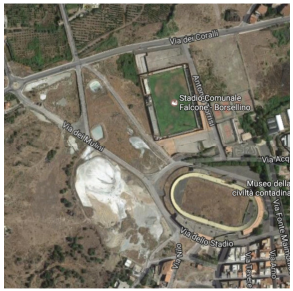
\includegraphics[width=0.3\paperwidth]{img/dump_map.png}}
    \end{center}
    \caption{Immagine satellitare dello scenario Illegal Dump.}
    \label{dump_map}
\end{figure}

\begin{figure}[H] 
    \captionsetup{justification=centering, margin=2cm, font=footnotesize}
    \begin{center}
    \makebox[\textwidth]{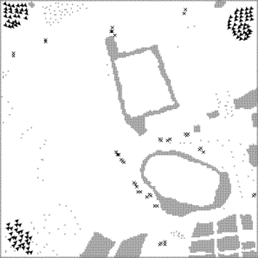
\includegraphics[width=0.3\paperwidth]{img/dump_scenario.png}}
    \end{center}
    \caption{Immagine vettoriale dello scenario Illegal Dump.}
    \label{dump_scenario}
\end{figure}

\subsection{Adattamento dell'algoritmo di esplorazione: SFE-RR1} \label{paragrafo_esplorazione_sciadro}

La configurazione dei parametri tecnologici utilizzata nella fase sperimentale dello scenario \textit{Illegal Dump} è illustrata di seguito e riassunta nella tabella \ref{tabella_parametri_dump}.

\begin{itemize}
    \item $algoritmo = SFE-RR \; 3.2$: la missione che viene simulata attraverso questo algoritmo è di tipo esplorativo; par tale motivo viene utilizzata la strategia di SFE con l'obiettivo principale di scoprire il $95 \%$ dei target distribuiti nell'area;
    \item $strategy = 3$: la logica di coordinamento comprende, in questo modo, stigmergia e flocking;
    \item $droneRadius = 0.2$: dalle specifiche tecniche del drone, il raggio è uguale a $0.3215 \; m = 0.1614 \; patch$;
    \item $speedMax = 8.5$: dalle specifiche tecniche del drone, la velocità massima in modalità professionale (che supporta il sistema di \textit{sense and avoid}) è uguale a $17 \; m/s = 8.534 \; patch/tick$;
    \item $cruisingSpeed = 2$: per garantire l'affidabilità del rilevamento dei sensori e per avere sufficiente spazio di frenata, il drone deve viaggiare ad una velocità non superiore a $13.8 \; m/s$. Per una maggiore sicurezza si limita tale velocità a $4 \; m/s = 2.008 \; patch/tick$;
    \item $acceleration = 2$, $deceleration = -2$: si considera un'accelerazione pari a $4.44 \; m/s^{2} = 2.229 \; patch/tick^{2}$;
    \item $angularVelMax = 2.6$: in relazione all'angolo di imbardata, il drone può raggiungere una velocità angolare massima di $2.618 \; rad/s$;
    \item $angularAcc = 7$, $angularDec = -7$: considerando la logica del simulatore ed il dato relativo alla velocità angolare del drone, si ottiene un'accelerazione angolare di $6.98 \; rad/s^{2}$;
    \item $endurance = 24$: viene considerata la durata minima della batteria di un drone del modello in esame;
    \item $sensingRadius = 2.5$: per calcolare questo valore, bisogna considerare una quota di volo pari a $10 \; m$;
    \item $sensingAngle = 360$;
    \item $reachableRadius = 4$: questo parametro rappresenta il raggio del settore circolare che il drone può prenotare ad ogni singola iterazione ed è collegato, di conseguenza, alla velocità di crociera;
    \item $reachableAngle = 360$: si considera un valore di \ang{360} al fine di garantire l'assenza di collisioni;
    \item $collisionVision = 6$: si deve considerare lo spazio di frenata necessario al drone per evitare la collisione, partendo dai parametri velocità ed accelerazione;
    \item $sightAngleMax = 60$: dalle specifiche tecniche del drone, il \textit{Field of View} è pari a \ang{60};
    \item $gapAngle = 20$: rappresenta l'angolo minimo necessario per l'attraversamento di un varco. 
\end{itemize}

\begin{table}[H]
    \centering
    \captionsetup{justification=centering, margin=2cm, font=footnotesize}
    \begin{tabular}{|l|c|}
    \hline
    \textbf{Parameter}              & \textbf{Value}                \\ \hline
    Radius                          & $0.2 \; patch$                \\ \hline
    Max speed                       & $8.5 \; patch/tick$           \\ \hline
    Cruising speed                  & $2 \; patch/tick$             \\ \hline
    Max acceleration                & $2 \; patch/tick^{2}$         \\ \hline
    Max deceleration                & $-2 \; patch/tick^{2}$        \\ \hline
    Max angular speed               & $2.6 \; rad/s$                \\ \hline
    Max angular acceleration        & $7 \; rad/s^{2}$              \\ \hline
    Max angular deceleration        & $-7 \; rad/s^{2}$             \\ \hline
    Battery duration                & $1440 \; tick$                \\ \hline
    Sensing radius                  & $2.5 \; patch$                \\ \hline
    Sensing angle                   & \ang{360}                        \\ \hline
    Reachable radius                & $4 \; patch$                  \\ \hline
    Reachable angle                 & \ang{360}                        \\ \hline
    Obstacle vision distance        & $6 \; patch$                  \\ \hline
    Obstacle vision angle           & \ang{60}                        \\ \hline
    Gap angle                       & \ang{20}                        \\ \hline
    \end{tabular}%
    
    \caption{Configurazione parametrica della tecnologia utilizzata nella fase sperimentale dello scenario \textit{Illegal Dump}.}
    \label{tabella_parametri_dump}
\end{table}

\subsubsection{Ottimizzazione parametrica con Differential Evolution}

Come indicato nel paragrafo \ref{sezione_de}, per la fase di ottimizzazione parametrica attraverso l'algoritmo di \textit{Differential Evolution}, è necessario fornire, oltre che i parametri da ottimizzare, anche degli intervalli che definiscono l'iperspazio all'interno del quale si effettua la ricerca dei valori ottimali.
Uno schema riassuntivo dei suddetti intervalli è presentato nella tabella \ref{tabella_intervalli_dump}

\begin{table}[H]
    \centering
    \captionsetup{justification=centering, margin=2cm, font=footnotesize}
    \begin{tabular}{|l|c|}
    \hline
    \textbf{Parameter}              & \textbf{Interval}                 \\ \hline
    radiusTop                       & $[1,13]$                          \\ \hline
    radiusDown                      & $[13,19]$                         \\ \hline
    evapRate                        & $[0.01,0.1]$                      \\ \hline
    olfaction                       & $[1,10]$                          \\ \hline
    flockAngle                      & $[15,45]$                         \\ \hline
    wiggleVar                       & $[5,15]$                          \\ \hline
    radiusSeparate                  & $[6,16]$                          \\ \hline
    maxSeparateTurn                 & $[30,45]$                         \\ \hline
    radiusAlign                     & $[16,22]$                         \\ \hline
    maxAlignTurn                    & $[30,45]$                         \\ \hline
    radiusCohere                    & $[18,26]$                         \\ \hline
maxCohereTurn                       & $[15,30]$                         \\ \hline
    \end{tabular}%
    
    \caption{Configurazione degli intervalli per l'ottimizzazione parametrica, attraverso l'algoritmo di \textit{Differential Evolution}, utilizzata nella fase sperimentale dello scenario \textit{Illegal Dump}.}
    \label{tabella_intervalli_dump}
\end{table}

Nel capitolo 5, abbiamo ampiamente illustrato le caratteristiche dell'algoritmo di DE.
In particolare, in questo caso avremo una popolazione di $NP$ elementi, dove ogni elemento è rappresentato da un vettore dei $D$ parametri da ottimizzare.
Nel caso specifico, com'è possibile osservare dalla tabella \ref{tabella_intervalli_dump}, $D=12$.

Per quanto riguarda $NP$, invece, in letteratura si trovano valori che vanno da $2D$ a $40D$.
Una popolazione grande, infatti, incrementa la possibilità di trovare la soluzione ottima, anche se ha un costo elevato in termini di tempo.
Per bilanciare questi due fattori, si è utilizzato un valore pari a $NP = 4D = 48$.

Infine, sono stati impostati sia gli iperparametri $F$ e $CR$, per le fasi di mutazione e crossover dell'algoritmo di DE, che la strategia di crossover.
Al fine di confrontare i risultati sperimentali di questo ambiente di simulazione con altri già effettuati sugli stessi scenari in \cite{cimino2019adaptive}, sono stati utilizzati gli stessi valori sia per il tasso di mutazione $F$ che per strategia e coefficiente di crossover $CR$.
In particolare:
\begin{itemize}
    \item \textit{Strategia di crossover:} DE/rand/1/bin;
    \item \textit{Tasso di mutazione:} $F=0.7$;
    \item \textit{Coefficiente di crossover:} $CR=0.5$
\end{itemize}

\subsubsection{Risultati sperimentali}

La strategia di \textit{SFE-RR} è stata implementata in NetLogo, una piattaforma di simulazione per \textit{Swarm Intelligence}.
L'ottimizzazione parametrica, invece, è stata costruita utilizzando la libreria \textit{SciPy} di \textit{Python}.

L'algoritmo di coordinamento dello sciame è stato testato sullo scenario \textit{Illegal Dump}, con la seguente strategia:
\begin{itemize}
    \item \textit{5 esecuzioni dell'algoritmo di Differential evolution;}
    \item \textit{3 ripetizione della simulazione per ogni elemento della popolazione;}
    \item \textit{Fitness function:} $f(x) = \# tick[95 \% \; target_{found}]$
\end{itemize}

\begin{figure}[H] 
    \captionsetup{justification=centering, margin=2cm, font=footnotesize}
    \begin{center}
        \makebox[0.5\paperwidth]{
            \begin{tikzpicture}
                \begin{axis}[
                    title={},
                    xlabel={Generazione},
                    ylabel={Tick},
                    xmin=0, xmax=40,
                    ymin=100, ymax=150,
                    xtick={5,10,15,20,25,30,35,40},
                    ytick={100,110,120,130,140,150},
                    legend pos=north east,
                    grid=major,
                    %ymajorgrids=true,
                    %xmajorgrids=true
                    %grid style=dashed,
                ]
                
                \addplot[
                    color=black,
                    line width=0.5mm,
                    ]
                    coordinates {
                        (1,130.58)(2,123.38)(3,120.18)(4,116.92)(5,115.4)(6,114.46)(7,114.46)(8,114.38)(9,114.04)(10,114.04)(11,112.66)(12,112.66)(13,112.66)(14,112.66)(15,111.8)(16,111.8)(17,111.8)(18,109.92)(19,108.92)(20,108.92)(21,108.92)(22,108.92)(23,108.92)(24,108.92)(25,108.92)(26,108.92)(27,108.92)(28,108.92)(29,108.92)(30,108.92)(31,108.92)(32,108.92)(33,108.92)(34,108.92)(35,108.92)(36,107.4)(37,107.4)(38,107.4)(39,107.4)(40,107.4)
                    };
                
                    \legend{\textit{average best fitness}}
                
                \end{axis}
            \end{tikzpicture}
        }
    \end{center}
    \caption{Ottimizzazione parametrica con Differential Evolution della strategia esplorativa di SFE, andamento della media tra le migliori fitness function delle 5 esecuzioni, al variare della generazione}
    \label{fitness_sciadro_dump}
\end{figure}   

\begin{table}[H]
    \centering
    \captionsetup{justification=centering, margin=2cm, font=footnotesize}
    \begin{tabular}{|l|c|}
    \hline
    \textbf{Algorithm}              & \textbf{Performance (tick)}              \\ \hline
    SFE-RR1        & $107.40 \; \pm \; 3.10$           \\ \hline
    \end{tabular}%
    
    \caption{Valutazione delle performance registrate dall'algoritmo di esplorazione di SFE-RR1.}
    \label{tabella_performance_dump}
\end{table}

\subsection{Adattamento dell'algoritmo di esplorazione: ACO-E}

La configurazione dei parametri tecnologici utilizzata per questa strategia è riassunta nella tabella \ref{tabella_parametri_dump_ACO}.
Per un'analisi dettagliata su tali parametri vedere il paragrafo \ref{esplorazione_paper}.

\begin{table}[H]
    \centering
    \captionsetup{justification=centering, margin=2cm, font=footnotesize}
    \begin{tabular}{|c|c|}
    \hline
    \textbf{Parameter}                      & \textbf{Value}        \\ \hline
    Wireless range                          & $100$                 \\ \hline
    $\beta_{0}$                             & $0.5$                 \\ \hline
    $\alpha$                                & $0.2$                 \\ \hline
    Inertial weight                         & $0.729$               \\ \hline
    Acceleration coefficient                & $2$                   \\ \hline
    \end{tabular}%
    
    \caption{Configurazione parametrica della tecnologia utilizzata nella fase sperimentale dello scenario \textit{Illegal Dump}.}
    \label{tabella_parametri_dump_ACO}
\end{table}
I parametri della tabella \ref{tabella_parametri_dump_ACO} sono stati impostati con i valori indicati in \cite{palmieri2017comparison}.

\subsubsection{Ottimizzazione parametrica con Differential Evolution}

Come previsto dall'algoritmo di \textit{Differential Evolution}, è necessario impostare degli intervalli che tale algoritmo utilizzerà durante l'ottimizzazione.
Sono stati definiti intervalli ampi per esplorare al meglio l'iperspazio definito dagli stessi.
In questo modo, infatti, si da più libertà all'algoritmo di DE di spaziare nella ricerca del minimo globale.

Lo schema riassuntivo degli intervalli utilizzato per la fase di ottimizzazione parametrica, nel caso della strategia di esplorazione \textit{ACO-E}, è presentato nella tabella \ref{tabella_intervalli_dump_ACO}

\begin{table}[H]
    \centering
    \captionsetup{justification=centering, margin=2cm, font=footnotesize}
    \begin{tabular}{|c|c|}
    \hline
    \textbf{Parameter}              & \textbf{Interval}         \\ \hline
    repulsiveStartIntensity         & $[0,100]$                 \\ \hline
    sensingRange                    & $[0,100]$                 \\ \hline
    EvaporationRateTimeUnit         & $[0,1]$                   \\ \hline
    $a_{1}$                         & $[0,2]$                   \\ \hline
    $a_{2}$                         & $[0,2]$                   \\ \hline
    $\phi$                          & $[0,2]$                   \\ \hline
    $\eta$                          & $[0,2]$                   \\ \hline
    $\lambda$                       & $[0,2]$                   \\ \hline
    \end{tabular}%
    
    \caption{Configurazione degli intervalli per l'ottimizzazione parametrica, attraverso l'algoritmo di \textit{Differential Evolution}, utilizzata nella fase sperimentale dello scenario \textit{Illegal Dump}.}
    \label{tabella_intervalli_dump_ACO}
\end{table}

Anche in questo caso, l'obiettivo è quello di effettuare un'analisi comparativa con le strategie utilizzate in precedenza.
A tal fine sono stati utilizzati gli stessi valori sia per il tasso di mutazione $F$ che per strategia e coefficiente di crossover $CR$.
In particolare:
\begin{itemize}
    \item \textit{Strategia di crossover:} DE/rand/1/bin;
    \item \textit{Tasso di mutazione:} $F=0.7$;
    \item \textit{Coefficiente di crossover:} $CR=0.5$
\end{itemize}

\subsubsection{Risultati sperimentali}

L'algoritmo di coordinamento esplorativo dello sciame è stato testato sullo scenario \textit{Illegal Dump}, con la seguente strategia:
\begin{itemize}
    \item \textit{5 esecuzioni dell'algoritmo di Differential evolution;}
    \item \textit{3 ripetizione della simulazione per ogni elemento della popolazione;}
    \item \textit{Fitness function:} $f(x) = \# tick[95 \% \; target_{found}]$
\end{itemize}

\begin{figure}[H] 
    \captionsetup{justification=centering, margin=2cm, font=footnotesize}
    \begin{center}
        \makebox[0.5\paperwidth]{
            \begin{tikzpicture}
                \begin{axis}[
                    title={},
                    xlabel={Generazione},
                    ylabel={Tick},
                    xmin=0, xmax=40,
                    ymin=150, ymax=200,
                    xtick={5,10,15,20,25,30,35,40},
                    ytick={150,160,170,180,190,200},
                    legend pos=north east,
                    grid=major,
                    %ymajorgrids=true,
                    %xmajorgrids=true
                    %grid style=dashed,
                ]
                
                \addplot[
                    color=black,
                    line width=0.5mm,
                    ]
                    coordinates {
                        (1,196.94)(2,187.48)(3,176.46)(4,173.94)(5,173.02)(6,172.48)(7,171.14)(8,169.42)(9,169.42)(10,168.88)(11,166.54)(12,166.48)(13,165.76)(14,165.7)(15,163.9)(16,163.7)(17,162.96)(18,162.22)(19,161.34)(20,161.34)(21,159.22)(22,159.22)(23,159.22)(24,159.22)(25,159.22)(26,155.08)(27,155)(28,155)(29,155)(30,155)(31,155)(32,155)(33,155)(34,153.54)(35,153.54)(36,153.54)(37,152.94)(38,152.94)(39,152.4)(40,150.86)
                    };
                
                    \legend{\textit{average best fitness}}
                
                \end{axis}
            \end{tikzpicture}
        }
    \end{center}
    \caption{Ottimizzazione parametrica con Differential Evolution della strategia esplorativa ACO-E, andamento della media tra le migliori fitness function delle 5 esecuzioni, al variare della generazione}
    \label{fitness_ACO_dump}
\end{figure}   

\begin{table}[H]
    \centering
    \captionsetup{justification=centering, margin=2cm, font=footnotesize}
    \begin{tabular}{|l|c|}
    \hline
    \textbf{Algorithm}              & \textbf{Performance (tick)}              \\ \hline
    ACO-E                & $161.34 \; \pm \; 6.21$           \\ \hline
    \end{tabular}%
    
    \caption{Valutazione delle performance registrate dall'algoritmo di esplorazione ACO-E.}
    \label{tabella_performance_dump_ACO}
\end{table}


\subsection{Adattamento dell'algoritmo di reclutamento: \\SFE-RR}

La strategia di reclutamento prevede una fase di lavorazione del target successiva alla scoperta dello stesso.
In questo caso, infatti, perché un target diventi \textit{Executed} è necessario che un numero minimo di droni si avvicini al target per l'esecuzione del task previsto dalla missione.

La configurazione dei parametri tecnologici utilizzata corrisponde con quella già introdotta nella sezione \ref{paragrafo_esplorazione_sciadro}.
L'unica differenza con il suddetto approccio di esplorazione è il parametro relativo al numero di droni necessario alla lavorazione del target, indicato con \textit{requiredDrones}.
Nelle fase sperimentale presentata di seguito $requiredDrones = 3$.

\subsubsection{Ottimizzazione parametrica con Differential Evolution}

Lo schema riassuntivo degli intervalli utilizzato nell'esecuzione dell'algoritmo di DE è presentato nella tabella \ref{tabella_intervalli_dump_sciadro32}

\begin{table}[H]
    \centering
    \captionsetup{justification=centering, margin=2cm, font=footnotesize}
    \begin{tabular}{|l|c|}
    \hline
    \textbf{Parameter}              & \textbf{Interval}                 \\ \hline
    radiusTop                       & $[1,13]$                          \\ \hline
    radiusDown                      & $[13,19]$                         \\ \hline
    evapRate                        & $[0.01,0.1]$                      \\ \hline
    olfaction                       & $[1,10]$                          \\ \hline
    flockAngle                      & $[15,45]$                         \\ \hline
    wiggleVar                       & $[5,15]$                          \\ \hline
    radiusSeparate                  & $[6,16]$                          \\ \hline
    maxSeparateTurn                 & $[30,45]$                         \\ \hline
    radiusAlign                     & $[16,22]$                         \\ \hline
    maxAlignTurn                    & $[30,45]$                         \\ \hline
    radiusCohere                    & $[18,26]$                         \\ \hline
maxCohereTurn                       & $[15,30]$                         \\ \hline
    \end{tabular}%
    
    \caption{Configurazione degli intervalli per l'ottimizzazione parametrica, attraverso l'algoritmo di \textit{Differential Evolution}, utilizzata nella fase sperimentale dello scenario \textit{Illegal Dump}.}
    \label{tabella_intervalli_dump_sciadro32}
\end{table}

Gli iperparametri $F$ e $CR$, per le fasi di mutazione e crossover dell'algoritmo di DE, e la strategia di crossover utilizzati sono illustrati di seguito:
\begin{itemize}
    \item \textit{Strategia di crossover:} DE/rand/1/bin;
    \item \textit{Tasso di mutazione:} $F=0.7$;
    \item \textit{Coefficiente di crossover:} $CR=0.5$
\end{itemize}

\subsubsection{Risultati sperimentali}

L'algoritmo di reclutamento è stato testato sullo scenario \textit{Illegal Dump}, con la seguente strategia:
\begin{itemize}
    \item \textit{5 esecuzioni dell'algoritmo di Differential evolution;}
    \item \textit{3 ripetizione della simulazione per ogni elemento della popolazione;}
    \item \textit{Fitness function:} $f(x) = \# tick[95 \% \; target_{executed}]$
\end{itemize}

\begin{figure}[H] 
    \captionsetup{justification=centering, margin=2cm, font=footnotesize}
    \begin{center}
        \makebox[0.5\paperwidth]{
            \begin{tikzpicture}
                \begin{axis}[
                    title={},
                    xlabel={Generazione},
                    ylabel={Tick},
                    xmin=0, xmax=40,
                    ymin=200, ymax=500,
                    xtick={5,10,15,20,25,30,35,40},
                    ytick={200,250,300,350,400,450,500},
                    legend pos=north east,
                    grid=major,
                    %ymajorgrids=true,
                    %xmajorgrids=true
                    %grid style=dashed,
                ]
                
                \addplot[
                    color=black,
                    line width=0.5mm,
                    ]
                    coordinates {
                        (1,474.6)(2,389.62)(3,381.68)(4,372.94)(5,372.94)(6,359.22)(7,339.6)(8,336.48)(9,317.28)(10,308.86)(11,285.34)(12,271.94)(13,271.94)(14,271.94)(15,271.94)(16,271.94)(17,271.94)(18,269.2)(19,262.26)(20,261.46)(21,261.46)(22,259.26)(23,258.52)(24,258.52)(25,257.8)(26,256)(27,253.26)(28,247.4)(29,236.4)(30,231.46)(31,231.46)(32,231.46)(33,227.72)(34,227.72)(35,227.72)(36,227.72)(37,223.24)(38,223.24)(39,222.04)(40,220.2)
                    };
                
                    \legend{\textit{average best fitness}}
                
                \end{axis}
            \end{tikzpicture}
        }
    \end{center}
    \caption{Ottimizzazione parametrica con Differential Evolution della strategia esplorativa di SFE, andamento della media tra le migliori fitness function delle 5 esecuzioni, al variare della generazione}
    \label{fitness_sciadro32_dump}
\end{figure}   

\begin{table}[H]
    \centering
    \captionsetup{justification=centering, margin=2cm, font=footnotesize}
    \begin{tabular}{|l|c|}
    \hline
    \textbf{Algorithm}              & \textbf{Performance (tick)}              \\ \hline
    SFE-RR3        & $220.20 \; \pm \; 15.13$           \\ \hline
    \end{tabular}%
    
    \caption{Valutazione delle performance registrate dall'algoritmo di reclutamento di SFE-RR5.}
    \label{tabella_performance_dump}
\end{table}

\subsection{Adattamento dell'algoritmo di reclutamento: \\ACO-ABC-RR-E}

Il solo dato relativo alla strategia di reclutamento di SFE-RR non è sufficiente per poterne trarre delle conclusioni.
A tal proposito, una procedura di ottimizzazione parametrica e valutazione dei risultati è stata effettuata anche sull'algoritmo \textit{Artificial Bee Colony for robot recruitment}, già ampiamente analizzato nei capitoli precedenti.
D'ora in avanti, la \textit{E} nel nome dell'algoritmo serve ad indicare l'applicazione dell'algoritmo di Evoluzione Differenziale alla strategia.

La configurazione dei parametri tecnologici utilizzata corrisponde con quella utilizzata nelle simulazioni inerenti l'algoritmo di reclutamento di SFE-RR.
Le uniche differenze riguardano i parametri legati alla strategia che sono riassunti di seguito:

\begin{table}[H]
    \centering
    \captionsetup{justification=centering, margin=2cm, font=footnotesize}
    \begin{tabular}{|c|c|}
    \hline
    \textbf{Parameter}                      & \textbf{Value}        \\ \hline
    $\beta_{0}$                             & $0.5$                 \\ \hline
    $\alpha$                                & $0.2$                 \\ \hline
    Inertial weight                         & $0.729$               \\ \hline
    Acceleration coefficient                & $2$                   \\ \hline
    \end{tabular}%
    
    \caption{Configurazione parametrica della tecnologia utilizzata nella fase sperimentale dello scenario \textit{Illegal Dump}.}
    \label{tabella_parametri_dump_ABC}
\end{table}
Vale la pena ricordare che tali parametri sono stati impostati come indicato in \cite{palmieri2017comparison}.

Nella fase sperimentale presentata di seguito $requiredDrones = 5$.

\subsubsection{Ottimizzazione parametrica con Differential Evolution}

Lo schema riassuntivo degli intervalli utilizzato nell'esecuzione dell'algoritmo di DE è presentato nella tabella \ref{tabella_intervalli_dump_ABC}.
Anche in questo caso si è deciso di mantenere degli intervalli ampi per non limitare l'esplorazione dell'algoritmo di ottimizzazione.

\begin{table}[H]
    \centering
    \captionsetup{justification=centering, margin=2cm, font=footnotesize}
    \begin{tabular}{|c|c|}
    \hline
    \textbf{Parameter}              & \textbf{Interval}                 \\ \hline
    wirelessRange                   & $[0,200]$                 \\ \hline
    repulsiveStartIntensity         & $[0,100]$                 \\ \hline
    sensingRange                    & $[0,100]$                 \\ \hline
    EvaporationRateTimeUnit         & $[0,1]$                   \\ \hline
    $a_{1}$                         & $[0,2]$                   \\ \hline
    $a_{2}$                         & $[0,2]$                   \\ \hline
    $\phi$                          & $[0,2]$                   \\ \hline
    $\eta$                          & $[0,2]$                   \\ \hline
    $\lambda$                       & $[0,2]$                   \\ \hline
    \end{tabular}%
    
    \caption{Configurazione degli intervalli per l'ottimizzazione parametrica, attraverso l'algoritmo di \textit{Differential Evolution}, utilizzata nella fase sperimentale dello scenario \textit{Illegal Dump}.}
    \label{tabella_intervalli_dump_ABC}
\end{table}

Gli iperparametri $F$ e $CR$, per le fasi di mutazione e crossover dell'algoritmo di DE, e la strategia di crossover utilizzati sono illustrati di seguito:
\begin{itemize}
    \item \textit{Strategia di crossover:} DE/rand/1/bin;
    \item \textit{Tasso di mutazione:} $F=0.7$;
    \item \textit{Coefficiente di crossover:} $CR=0.5$
\end{itemize}

\subsubsection{Risultati sperimentali}

L'algoritmo di reclutamento è stato testato sullo scenario \textit{Illegal Dump}, con la seguente strategia:
\begin{itemize}
    \item \textit{5 esecuzioni dell'algoritmo di Differential evolution;}
    \item \textit{3 ripetizione della simulazione per ogni elemento della popolazione;}
    \item \textit{Fitness function:} $f(x) = \# tick[95 \% \; target_{executed}]$
\end{itemize}

\begin{figure}[H] 
    \captionsetup{justification=centering, margin=2cm, font=footnotesize}
    \begin{center}
        \makebox[0.5\paperwidth]{
            \begin{tikzpicture}
                \begin{axis}[
                    title={},
                    xlabel={Generazione},
                    ylabel={Tick},
                    xmin=0, xmax=40,
                    ymin=250, ymax=500,
                    xtick={5,10,15,20,25,30,35,40},
                    ytick={250,300,350,400,450,500},
                    legend pos=north east,
                    grid=major,
                    %ymajorgrids=true,
                    %xmajorgrids=true
                    %grid style=dashed,
                ]
                
                \addplot[
                    color=black,
                    line width=0.5mm,
                    ]
                    coordinates {
                        (1,469.24)(2,384.58)(3,338.06)(4,332.08)(5,312.42)(6,301.48)(7,299)(8,298.2)(9,294.14)(10,289.12)(11,289.12)(12,288.46)(13,285.2)(14,282.72)(15,281.26)(16,281.26)(17,281.26)(18,281.26)(19,279.46)(20,279.46)(21,278.34)(22,278.34)(23,278.34)(24,278.34)(25,277.88)(26,277.88)(27,277.88)(28,275.28)(29,275.28)(30,275.28)(31,275.28)(32,275.28)(33,275.28)(34,275.28)(35,275.28)(36,275.28)(37,275.28)(38,275.28)(39,275.28)(40,275.28)
                    };
                
                    \legend{\textit{average best fitness}}
                
                \end{axis}
            \end{tikzpicture}
        }
    \end{center}
    \caption{Ottimizzazione parametrica con Differential Evolution della strategia esplorativa di SFE, andamento della media tra le migliori fitness function delle 5 esecuzioni, al variare della generazione}
    \label{fitness_sciadro32_dump}
\end{figure}   

\begin{table}[H]
    \centering
    \captionsetup{justification=centering, margin=2cm, font=footnotesize}
    \begin{tabular}{|l|c|}
    \hline
    \textbf{Algorithm}              & \textbf{Performance (tick)}              \\ \hline
    ACO-ABC-RR3-E                & $275.28 \; \pm \; 3.87$           \\ \hline
    \end{tabular}%
    
    \caption{Valutazione delle performance registrate dall'algoritmo di reclutamento ACO-ABC-RR5-E.}
    \label{tabella_performance_dump}
\end{table}

\section{Scenario \textit{Rural Mine}}

Lo scenario è statico: \textit{Rural Mine} si basa su dati di pubblico dominio relativi a mine antiuomo presenti in aree extraurbane vicino Sarajevo, Bosnia-Herzegovina \cite{seedemining2018}.
Di seguito sono riportate le caratteristiche dello scenario:

\begin{itemize}
    \item \textit{Area in metri:} 400 x 400
    \item \textit{Area in patch:} 201 x 201
    \item \textit{Dimensione patch:} 1.99m x 1.99m
    \item \textit{Conversione spaziale:} 1 m = 0.502 patch
    \item \textit{Conversione temporale:} 1 s = 1 tick
    \item \textit{Numero target statici presenti nell'area:} 28
    \item \textit{Numero target dinamici presenti nell'area:} 0
    \item \textit{Numero ostacoli presenti nell'area:} 285
    \item \textit{Flotta utilizzata:} 80 droni
\end{itemize}

Lo scenario presenta solo target statici, di conseguenza la funzione obiettivo è rappresentata dal tempo di rilevamento del $95 \%$ dei target.

Per osservarne la complessità ambientale, le figure \ref{ruralMine_map} e \ref{ruralMine_scenario} mostrano la mappa satellitare utilizzata per \textit{Rural Mine}, e la corrispondente immagine vettoriale iniziale rappresentata nell'ambiente di simulazione, rispettivamente. 
Gli ostacoli  sono rappresentati in grigio, mentre i bersagli sono rappresentati come 'x' nere. 
I droni sono posizionati agli angoli e sono orientati verso il centro dell'area.

\begin{figure}[H] 
    \captionsetup{justification=centering, margin=2cm, font=footnotesize}
    \begin{center}
    \makebox[\textwidth]{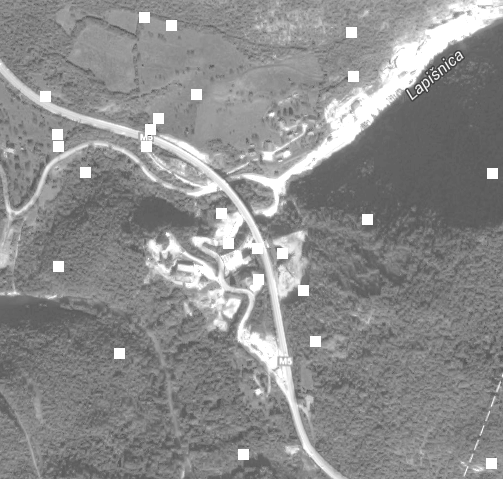
\includegraphics[width=0.3\paperwidth]{img/ruralMine_map.png}}
    \end{center}
    \caption{Immagine satellitare dello scenario Rural Mine.}
    \label{ruralMine_map}
\end{figure}

\begin{figure}[H] 
    \captionsetup{justification=centering, margin=2cm, font=footnotesize}
    \begin{center}
    \makebox[\textwidth]{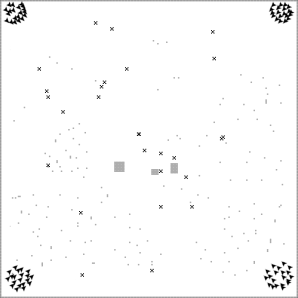
\includegraphics[width=0.3\paperwidth]{img/ruralMine_scenario.png}}
    \end{center}
    \caption{Immagine vettoriale dello scenario Rural Mine.}
    \label{ruralMine_scenario}
\end{figure}

La configurazione dei parametri tecnologici utilizzata nella fase sperimentale dello scenario \textit{Rural Mine} è  riassunta nella tabella \ref{tabella_parametri_ruralMine}.

\begin{table}[H]
    \centering
    \captionsetup{justification=centering, margin=2cm, font=footnotesize}
    \begin{tabular}{|l|c|}
    \hline
    \textbf{Parameter}              & \textbf{Value}                \\ \hline
    Radius                          & $0.2 \; patch$                \\ \hline
    Max speed                       & $8.5 \; patch/tick$           \\ \hline
    Cruising speed                  & $2 \; patch/tick$             \\ \hline
    Max acceleration                & $2 \; patch/tick^{2}$         \\ \hline
    Max deceleration                & $-2 \; patch/tick^{2}$        \\ \hline
    Max angular speed               & $2.6 \; rad/s$                \\ \hline
    Max angular acceleration        & $7 \; rad/s^{2}$              \\ \hline
    Max angular deceleration        & $-7 \; rad/s^{2}$             \\ \hline
    Battery duration                & $1440 \; tick$                \\ \hline
    Sensing radius                  & $2.5 \; patch$                \\ \hline
    Sensing angle                   & \ang{360}                        \\ \hline
    Reachable radius                & $4 \; patch$                  \\ \hline
    Reachable angle                 & \ang{360}                        \\ \hline
    Obstacle vision distance        & $6 \; patch$                  \\ \hline
    Obstacle vision angle           & \ang{60}                        \\ \hline
    Gap angle                       & \ang{20}                        \\ \hline
    \end{tabular}%
    
    \caption{Configurazione parametrica della tecnologia utilizzata nella fase sperimentale dello scenario \textit{Rural Mine}.}
    \label{tabella_parametri_ruralMine}
\end{table}

\subsection{Ottimizzazione parametrica con Differential Evolution}

Uno schema riassuntivo degli intervalli utilizzati per la fase di ottimizzazione parametrica attraverso l'algoritmo di \textit{Differential Evolution} è presentato nella tabella \ref{tabella_intervalli_ruralMine}
La scelta di tali intervalli è il risultato di una prima fase di ottimizzazione parametrica utilizzando gli intervalli mostrati nella tabella \ref{tabella_intervalli_dump}.
Al fine di approfondire lo studio del minimo ottenuto dalla suddetta fase, si è deciso di effettuare un nuovo studio nell'iperspazio identificato dagli intervalli mostrati di seguito.

\begin{table}[H]
    \centering
    \captionsetup{justification=centering, margin=2cm, font=footnotesize}
    \begin{tabular}{|l|c|}
    \hline
    \textbf{Parameter}              & \textbf{Interval}                 \\ \hline
    radiusTop                       & $[5.13,7.73]$                          \\ \hline
    radiusDown                      & $[17.29,18.69]$                         \\ \hline
    evapRate                        & $[0.037,0.057]$                      \\ \hline
    olfaction                       & $[2.67,4.67]$                          \\ \hline
    flockAngle                      & $[17.31,23.51]$                         \\ \hline
    wiggleVar                       & $[10.32,12.52]$                          \\ \hline
    radiusSeparate                  & $[10.15,12.35]$                          \\ \hline
    maxSeparateTurn                 & $[32.32,35.52]$                         \\ \hline
    radiusAlign                     & $[16.70,18.10]$                         \\ \hline
    maxAlignTurn                    & $[40.93,44.13]$                         \\ \hline
    radiusCohere                    & $[18.54,20.34]$                         \\ \hline
    maxCohereTurn                   & $[26.72,29.92]$                         \\ \hline
    \end{tabular}%
    
    \caption{Configurazione degli intervalli per l'ottimizzazione parametrica, attraverso l'algoritmo di \textit{Differential Evolution}, utilizzata nella fase sperimentale dello scenario \textit{Rural Mine}.}
    \label{tabella_intervalli_ruralMine}
\end{table}

I valori relativi agli iperparametri sono i seguenti:
\begin{itemize}
    \item \textit{Strategia di crossover:} DE/rand/1/bin;
    \item \textit{Tasso di mutazione:} $F=0.7$;
    \item \textit{Coefficiente di crossover:} $CR=0.5$
\end{itemize}

\subsection{Risultati sperimentali}

L'algoritmo di coordinamento dello sciame è stato testato sullo scenario \textit{Rural Mine}, con la seguente strategia:
\begin{itemize}
    \item \textit{5 esecuzioni dell'algoritmo di Differential evolution;}
    \item \textit{3 ripetizione della simulazione per ogni elemento della popolazione;}
    \item \textit{Fitness function:} $f(x) = \# tick[95 \% \; target_{found}]$
\end{itemize}

\begin{figure}[H] 
    \captionsetup{justification=centering, margin=2cm, font=footnotesize}
    \begin{center}
        \makebox[0.5\paperwidth]{
            \begin{tikzpicture}
                \begin{axis}[
                    title={},
                    xlabel={Generazione},
                    ylabel={Tick},
                    xmin=0, xmax=40,
                    ymin=120, ymax=150,
                    xtick={5,10,15,20,25,30,35,40},
                    ytick={120,125,130,135,140,145,150},
                    legend pos=north east,
                    grid=major,
                    %ymajorgrids=true,
                    %xmajorgrids=true
                    %grid style=dashed,
                ]
                
                \addplot[
                    color=black,
                    line width=0.5mm,
                    ]
                    coordinates {
                        (1,148.2)(2,143)(3,139.28)(4,137.22)(5,135.34)(6,131.46)(7,130.52)(8,129.6)(9,129.6)(10,127.66)(11,124.4)(12,124.4)(13,124.4)(14,124.4)(15,124.4)(16,122.34)(17,122.34)(18,122.34)(19,122.34)(20,122.34)(21,122.34)(22,122.34)(23,122.34)(24,122.34)(25,122.34)(26,122.2)(27,121.26)(28,121.26)(29,121.26)(30,120.32)(31,120.32)(32,120.32)(33,120.32)(34,120.32)(35,120.32)(36,120.32)(37,120.32)(38,120.32)(39,120.32)(40,120.32)
                    };
                
                    \legend{\textit{average best fitness}}
                
                \end{axis}
            \end{tikzpicture}
        }
    \end{center}
    \caption{Ottimizzazione parametrica con Differential Evolution, andamento della media tra le migliori fitness function delle 5 esecuzioni, al variare della generazione}
    \label{fitness_sciadro_ruralMine}
\end{figure}   

\begin{table}[H]
    \centering
    \captionsetup{justification=centering, margin=2cm, font=footnotesize}
    \begin{tabular}{|l|c|}
    \hline
    \textbf{Algorithm}              & \textbf{Performance (tick)}       \\ \hline
    SFE-RR1                     & $120.32 \; \pm \; 4.91$           \\ \hline
    \end{tabular}%
    
    \caption{Valutazione delle performance registrate dall'algoritmo di esplorazione di SFE-RR1.}
    \label{tabella_performance_ruralMine}
\end{table}

\section{Scenario \textit{Urban Mine}}

Lo scenario è statico: \textit{Urban Mine} si basa su dati di pubblico dominio relativi a mine antiuomo presenti in aree urbane vicino Sarajevo, Bosnia-Herzegovina \cite{seedemining2018}.
Di seguito sono riportate le caratteristiche dello scenario:

\begin{itemize}
    \item \textit{Area in metri:} 400 x 400
    \item \textit{Area in patch:} 201 x 201
    \item \textit{Dimensione patch:} 1.99m x 1.99m
    \item \textit{Conversione spaziale:} 1 m = 0.502 patch
    \item \textit{Conversione temporale:} 1 s = 1 tick
    \item \textit{Numero target statici presenti nell'area:} 40
    \item \textit{Numero target dinamici presenti nell'area:} 0
    \item \textit{Numero ostacoli presenti nell'area:} 3664
    \item \textit{Flotta utilizzata:} 80 droni
\end{itemize}

Lo scenario presenta solo target statici, di conseguenza la funzione obiettivo è rappresentata dal tempo di rilevamento del $95 \%$ dei target.

Per osservarne la complessità ambientale, le figure \ref{urbanMine_map} e \ref{urbanMine_scenario} mostrano la mappa satellitare utilizzata per \textit{Urban Mine}, e la corrispondente immagine vettoriale iniziale rappresentata nell'ambiente di simulazione, rispettivamente. 
Gli ostacoli  sono rappresentati in grigio, mentre i bersagli sono rappresentati come 'x' nere. 
I droni sono posizionati agli angoli e sono orientati verso il centro dell'area.

\begin{figure}[H] 
    \captionsetup{justification=centering, margin=2cm, font=footnotesize}
    \begin{center}
    \makebox[\textwidth]{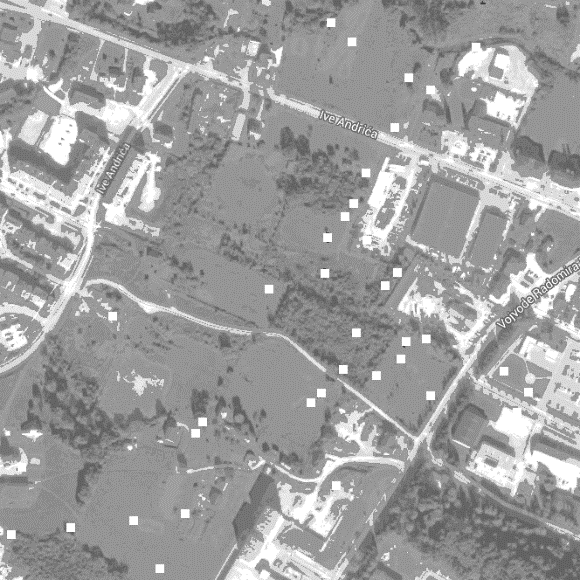
\includegraphics[width=0.3\paperwidth]{img/urbanMine_map.png}}
    \end{center}
    \caption{Immagine satellitare dello scenario Urban Mine.}
    \label{urbanMine_map}
\end{figure}

\begin{figure}[H] 
    \captionsetup{justification=centering, margin=2cm, font=footnotesize}
    \begin{center}
    \makebox[\textwidth]{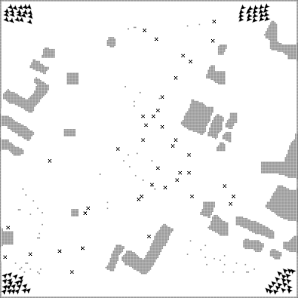
\includegraphics[width=0.3\paperwidth]{img/urbanMine_scenario.png}}
    \end{center}
    \caption{Immagine vettoriale dello scenario Urban Mine.}
    \label{urbanMine_scenario}
\end{figure}

La configurazione dei parametri tecnologici utilizzata nella fase sperimentale dello scenario \textit{Urban Mine} è  riassunta nella tabella \ref{tabella_parametri_urbanMine}.

\begin{table}[H]
    \centering
    \captionsetup{justification=centering, margin=2cm, font=footnotesize}
    \begin{tabular}{|l|c|}
    \hline
    \textbf{Parameter}              & \textbf{Value}                \\ \hline
    Radius                          & $0.2 \; patch$                \\ \hline
    Max speed                       & $8.5 \; patch/tick$           \\ \hline
    Cruising speed                  & $2 \; patch/tick$             \\ \hline
    Max acceleration                & $2 \; patch/tick^{2}$         \\ \hline
    Max deceleration                & $-2 \; patch/tick^{2}$        \\ \hline
    Max angular speed               & $2.6 \; rad/s$                \\ \hline
    Max angular acceleration        & $7 \; rad/s^{2}$              \\ \hline
    Max angular deceleration        & $-7 \; rad/s^{2}$             \\ \hline
    Battery duration                & $1440 \; tick$                \\ \hline
    Sensing radius                  & $2.5 \; patch$                \\ \hline
    Sensing angle                   & \ang{360}                        \\ \hline
    Reachable radius                & $4 \; patch$                  \\ \hline
    Reachable angle                 & \ang{360}                        \\ \hline
    Obstacle vision distance        & $6 \; patch$                  \\ \hline
    Obstacle vision angle           & \ang{60}                        \\ \hline
    Gap angle                       & \ang{20}                        \\ \hline
    \end{tabular}%
    
    \caption{Configurazione parametrica della tecnologia utilizzata nella fase sperimentale dello scenario \textit{Urban Mine}.}
    \label{tabella_parametri_urbanMine}
\end{table}

\subsection{Ottimizzazione parametrica con Differential Evolution}

Uno schema riassuntivo degli intervalli utilizzati per la fase di ottimizzazione parametrica attraverso l'algoritmo di \textit{Differential Evolution} è presentato nella tabella \ref{tabella_intervalli_urbanMine}.
Anche in questo caso, la scelta degli intervalli è frutto di uno studio precedente sugli intervalli della tabella \ref{tabella_intervalli_dump}.

\begin{table}[H]
    \centering
    \captionsetup{justification=centering, margin=2cm, font=footnotesize}
    \begin{tabular}{|l|c|}
    \hline
    \textbf{Parameter}              & \textbf{Interval}                 \\ \hline
    radiusTop                       & $[1,13]$                          \\ \hline
    radiusDown                      & $[13,19]$                         \\ \hline
    evapRate                        & $[0.01,0.1]$                      \\ \hline
    olfaction                       & $[1,10]$                          \\ \hline
    flockAngle                      & $[15,45]$                         \\ \hline
    wiggleVar                       & $[5,15]$                          \\ \hline
    radiusSeparate                  & $[6,16]$                          \\ \hline
    maxSeparateTurn                 & $[30,45]$                         \\ \hline
    radiusAlign                     & $[16,22]$                         \\ \hline
    maxAlignTurn                    & $[30,45]$                         \\ \hline
    radiusCohere                    & $[18,26]$                         \\ \hline
    maxCohereTurn                   & $[15,30]$                         \\ \hline
    \end{tabular}%
    
    \caption{Configurazione degli intervalli per l'ottimizzazione parametrica, attraverso l'algoritmo di \textit{Differential Evolution}, utilizzata nella fase sperimentale dello scenario \textit{Urban Mine}.}
    \label{tabella_intervalli_urbanMine}
\end{table}

I valori relativi agli iperparametri sono i seguenti:
\begin{itemize}
    \item \textit{Strategia di crossover:} DE/rand/1/bin;
    \item \textit{Tasso di mutazione:} $F=0.7$;
    \item \textit{Coefficiente di crossover:} $CR=0.5$
\end{itemize}

\subsection{Risultati sperimentali}

L'algoritmo di coordinamento dello sciame è stato testato sullo scenario \textit{Urban Mine}, con la seguente strategia:
\begin{itemize}
    \item \textit{5 esecuzioni dell'algoritmo di Differential evolution;}
    \item \textit{3 ripetizione della simulazione per ogni elemento della popolazione;}
    \item \textit{Fitness function:} $f(x) = \# tick[95 \% \; target_{found}]$
\end{itemize}

\begin{figure}[H] 
    \captionsetup{justification=centering, margin=2cm, font=footnotesize}
    \begin{center}
        \makebox[0.5\paperwidth]{
            \begin{tikzpicture}
                \begin{axis}[
                    title={},
                    xlabel={Generazione},
                    ylabel={Tick},
                    xmin=0, xmax=40,
                    ymin=150, ymax=200,
                    xtick={5,10,15,20,25,30,35,40},
                    ytick={150,160,170,180,190,200},
                    legend pos=north east,
                    grid=major,
                    %ymajorgrids=true,
                    %xmajorgrids=true
                    %grid style=dashed,
                ]
                
                \addplot[
                    color=black,
                    line width=0.5mm,
                    ]
                    coordinates {
                        (1,195.94)(2,186.82)(3,175.54)(4,174.6)(5,174.6)(6,169.94)(7,167.86)(8,167.86)(9,167.86)(10,167.86)(11,166.2)(12,165.8)(13,165.8)(14,165.8)(15,163.94)(16,160.34)(17,160.34)(18,160.34)(19,160.34)(20,160.34)(21,160.34)(22,160.34)(23,160.34)(24,160.34)(25,160.34)(26,160.34)(27,160.34)(28,160.34)(29,160.34)(30,158.74)(31,158.74)(32,158.74)(33,158.74)(34,158.74)(35,158.74)(36,158.74)(37,158.74)(38,156.74)(39,156.74)(40,156.74)
                    };
                
                    \legend{\textit{average best fitness}}
                
                \end{axis}
            \end{tikzpicture}
        }
    \end{center}
    \caption{Ottimizzazione parametrica con Differential Evolution, andamento della media tra le migliori fitness function delle 5 esecuzioni, al variare della generazione}
    \label{fitness_sciadro_urbanMine}
\end{figure}   

\begin{table}[H]
    \centering
    \captionsetup{justification=centering, margin=2cm, font=footnotesize}
    \begin{tabular}{|l|c|}
    \hline
    \textbf{Algorithm}              & \textbf{Performance (tick)}       \\ \hline
    SFE-RR1                     & $160.34 \; \pm \; 5.42$           \\ \hline
    \end{tabular}%
    
    \caption{Valutazione delle performance registrate dall'algoritmo di esplorazione di SFE-RR1.}
    \label{tabella_performance_urbanMine}
\end{table}

\newpage
\section{Analisi comparativa delle performance}

In questa sezione verrà presentato uno schema riassuntivo dei risultati ottenuti nella fase sperimentale, al fine di poter effettuare una comparazione tra le performance registrate dalle varie strategie adottate.

Per lo scenario \textit{Illegal Dump} sono state adattate entrambe le strategie di esplorazione introdotte nei capitoli precedenti e sono state confrontate con i risultati di altri studi presenti in letteratura.
La tabella \ref{analisi_comparativa_esplorazione_dump} mostra i risultati degli esperimenti realizzati.

Per il calcolo della durata di ogni singola ottimizzazione utilizziamo la seguente notazione:
\begin{itemize}
    \item $S:$ durata di una simulazione;
    \item $N:$ numero individui della popolazione utilizzata dal DE;
    \item $G:$ numero di generazioni totali del DE;
\end{itemize}
Consideriamo adesso le seguenti durate, in media, delle simulazioni sui vari scenari, per SFE e SFE-RR1:
\begin{itemize}
    \item \textit{Illegal Dump: }$S = 50s$;
    \item \textit{Rural Mine: }$S = 44s$;
    \item \textit{Urban Mine: }$S = 49s$;
\end{itemize}
Per ACO-E, invece, la durata media delle simulazioni sullo scenario \textit{Illegal Dump} è pari a $S = 80s$.
In tutte le ottimizzazioni eseguite, $G=40$.

Per quanto riguarda il numero di individui della popolazione, invece, esso dipende dalla strategia adottata:
\begin{itemize}
    \item SFE: $N = 40$;
    \item SFE-RR1: $N = 48$;
    \item ACO-E: $N = 32$
\end{itemize}

A questo punto, la durata sarà uguale a:
\begin{equation*}
    duration = \begin{cases}
        S \cdot N \cdot G \; , \; \text{in caso di ottimizzazione serializzata}\\
        S  \cdot G \; , \; \text{in caso di ottimizzazione parallelizzata}
    \end{cases}   
\end{equation*}

\begin{table}[H]
    \centering
    \captionsetup{justification=centering, margin=2cm, font=footnotesize}
    \begin{tabular}{|l|c|c|}
    \hline
    \textbf{Algorithm}              & \textbf{Performance (tick)}       & \textbf{Optimization duration}      \\ \hline
    SFE                             & $121.70 \; \pm \; 4.75$           & $22.22 \; h$                                      \\ \hline
    SFE-RR1                         & $107.40 \; \pm \; 3.10$           & $0.55 \; h$                                       \\ \hline
    ACO-E                           & $161.34 \; \pm \; 6.21$           & $0.89 \; h$                                     \\ \hline
    \end{tabular}%
    
    \caption{Strategia di esplorazione dello scenario \textit{Illegal Dump}, analisi comparativa delle performance.}
    \label{analisi_comparativa_esplorazione_dump}
\end{table}

Come si evince da tali risultati sullo scenario \textit{Illegal Dump}, il nuovo approccio supera sensibilmente sia le performance ottenute in \cite{cimino2019adaptive}, sia l'adattamento dell'algoritmo implementato in \cite{palmieri2017comparison}, accuratamente integrato nel simulation testbed.
SFE-RR1, infatti, migliora le performance di missione di circa il 97\% rispetto a SFE e del 96\% rispetto ad ACO-E, con tempi di durata dell'ottimizzazione molto minori (approssimativamente il 93\% in meno rispetto a SFE e l'83\% rispetto a ACO-E).

Per quanto riguarda le strategie di reclutamento, invece, i risultati prodotti dalle varie esecuzioni del simulatore sono riassunti nella tabella \ref{analisi_comparativa_reclutamento_dump}.

\begin{table}[H]
    \centering
    \captionsetup{justification=centering, margin=2cm, font=footnotesize}
    \begin{tabular}{|l|c|}
    \hline
    \textbf{Algorithm}              & \textbf{Performance (tick)}       \\ \hline
    SFE-RR3                         & $220.20 \; \pm \; 15.13$           \\ \hline
    ACO-ABC-RR3-E                   & $275.28 \; \pm \; 3.87$           \\ \hline
    \end{tabular}%
    
    \caption{Strategia di reclutamento nello scenario \textit{Illegal Dump}, analisi comparativa delle performance.}
    \label{analisi_comparativa_reclutamento_dump}
\end{table}

Anche in questo caso, le metaeuristiche utilizzate nell'approccio SFE-RR hanno prodotto risultati interessanti, soprattutto in relazione a quanto ottenuto dall'integrazione, adattamento e simulazione della strategia ACO-ABC-RR5-E.
Le performance della strategia di esplorazione e reclutamento SFE-RR5, infatti, risulta migliore dell'approccio ACO-ABC-RR5-E di circa il 20\%.

Per gli scenari \textit{Rural Mine} e \textit{Urban Mine} si è scelto di adattare solo la strategia di esplorazione SFE-RR1, al fine di testarne le performance su scenari di diverse conformazioni.
Anche in questo caso si è scelto di valutare le performance del simulatore attraverso un confronto con le performance registrate, sugli stessi scenari, da SFE.
Le tabelle \ref{analisi_comparativa_esplorazione_ruralMine} e \ref{analisi_comparativa_esplorazione_urbanMine} mostrano i risultati degli esperimenti realizzati.

\begin{table}[H]
    \centering
    \captionsetup{justification=centering, margin=2cm, font=footnotesize}
    \begin{tabular}{|l|c|c|}
    \hline
    \textbf{Algorithm}              & \textbf{Performance (tick)}       & \textbf{Optimization duration}      \\ \hline
    SFE                             & $125.96 \; \pm \; 8.90$           &$19.55 \; h$       \\ \hline
    SFE-RR1                         & $120.32 \; \pm \; 4.91$           &$0.49  \; h$       \\ \hline
    \end{tabular}%
    
    \caption{Strategia di esplorazione dello scenario \textit{Rural Mine}, analisi comparativa delle performance.}
    \label{analisi_comparativa_esplorazione_ruralMine}
\end{table}

\begin{table}[H]
    \centering
    \captionsetup{justification=centering, margin=2cm, font=footnotesize}
    \begin{tabular}{|l|c|c|}
    \hline
    \textbf{Algorithm}              & \textbf{Performance (tick)}       & \textbf{Optimization duration}      \\ \hline
    SFE                             & $152.38 \; \pm \; 5.25$           &$21.78 \; h$       \\ \hline
    SFE-RR1                         & $160.34 \; \pm \; 5.42$           &$0.54  \; h$       \\ \hline
    \end{tabular}%
    
    \caption{Strategia di esplorazione dello scenario \textit{Urban Mine}, analisi comparativa delle performance.}
    \label{analisi_comparativa_esplorazione_urbanMine}
\end{table}

Nei due scenari riguardanti le missioni di sminamento, la strategia di SFE-RR1 è riuscita a raggiungere performance simili a quanto già prodotto in SFE.

\`E fondamentale sottolineare, ad ogni modo, che il nuovo meccanismo di ottimizzazione parametrica prevede un'esecuzione parallelizzata dell'algoritmo di Differential Evolution.
Questo si traduce in un costo molto minore in termini di tempo necessario al completamento del task, rispetto all'esecuzione dello stesso algoritmo in Matlab, come si evince dalla durata delle ottimizzazioni indicata nelle tabelle \ref{analisi_comparativa_esplorazione_dump}, \ref{analisi_comparativa_esplorazione_ruralMine} e \ref{analisi_comparativa_esplorazione_urbanMine}.
Il miglioramento di tali prestazioni, infatti, è pari a circa il 97\% in entrambi gli scenari.

\newpage
\section{Conclusioni}

Il documento riassume la progettazione di un ambiente di simulazione per l’integrazione di approcci bio-ispirati per il coordinamento degli UAV coinvolti nel rilevamento e nel monitoraggio dei target distribuiti. 
La logica di coordinamento comprende un'autoformazione spaziale e una collaborazione basata su comunicazioni dirette e indirette tra gli attori della missione. 
Lo sciame, inoltre, adatta i suoi parametri alla missione specifica utilizzando un algoritmo di ottimizzazione basato su evoluzione differenziale. 

Gli esperimenti sono incoraggianti, in quanto l'approccio proposto si estende e, in alcuni casi, supera approcci simile in letteratura. 
La possibilità di parallelizzare i calcoli eseguiti dall'algoritmo di Differential Evolution, infatti, si è dimostrato molto più efficiente in termini di performance temporali.
La durata di una completa esecuzione del meccanismo di ottimizzazione, infatti, passa dalle 22 ore circa a durate dell'ordine dell'ora, con un risultato simile o migliore in termini di prestazioni dello sciame.

Un ulteriore miglioramento delle prestazioni si potrebbe ottenere dallo studio degli iperparametri del DE: i parametri utilizzati in fase sperimentale, infatti, vanno ad influenzare il cammino all'interno dell'iperspazio definito dagli intervalli dei parametri da ottimizzare.
Andando ad abbassare i parametri \textit{F} e \textit{CR}, infatti, potremmo sì rallentare la convergenza, ma anche esplorare in modo migliore l'iperspazio alla ricerca del minimo globale o, comunque, di un punto ad esso vicino.
Le performance garantite da questo nuovo approccio parallelizzato ci danno, altresì, la possibilità di allargare gli intervalli in cui spaziare e di avere, in ogni caso, esecuzioni con durata inferiore alle 2 ore. 

Il lavoro futuro potrebbe, dunque, consistere nell’approfondire le funzionalità adattive del simulatore ed integrare nuovi scenari e nuove strategie per fornire ulteriori risultati comparativi, al fine di validare le caratteristiche strutturali dell’ambiente di simulazione.
\chapter*{Ringraziamenti}


\bibliography{bibliography} 
\bibliographystyle{ieeetr}

\end{document}